%%%%%%%%%%%%%%%%%%%%%%%%%%%%%%%%%%%%%%%%%
% Beamer Presentation
% LaTeX Template
% Version 1.0 (10/11/12)
%
% This template has been downloaded from:
% http://www.LaTeXTemplates.com
%
% License:
% CC BY-NC-SA 3.0 (http://creativecommons.org/licenses/by-nc-sa/3.0/)
%
%%%%%%%%%%%%%%%%%%%%%%%%%%%%%%%%%%%%%%%%%

%----------------------------------------------------------------------------------------
%	PACKAGES AND THEMES
%----------------------------------------------------------------------------------------

\documentclass{beamer}

\mode<presentation> {

% The Beamer class comes with a number of default slide themes
% which change the colors and layouts of slides. Below this is a list
% of all the themes, uncomment each in turn to see what they look like.

% \usetheme{default}
%\usetheme{AnnArbor}
%\usetheme{Antibes}
%\usetheme{Bergen}
% \usetheme{Berkeley}
%\usetheme{Berlin}
%\usetheme{Boadilla}
%\usetheme{CambridgeUS}
%\usetheme{Copenhagen}
%\usetheme{Darmstadt}
%\usetheme{Dresden}
%\usetheme{Frankfurt}
%\usetheme{Goettingen}
%\usetheme{Hannover}
%\usetheme{Ilmenau}
%\usetheme{JuanLesPins}
%\usetheme{Luebeck}
%\usetheme{Madrid}
%\usetheme{Malmoe}
%\usetheme{Marburg}
%\usetheme{Montpellier}
%\usetheme{PaloAlto}
%\usetheme{Pittsburgh}
%\usetheme{Rochester}
%\usetheme{Singapore}
%\usetheme{Szeged}
%\usetheme{Warsaw}

% As well as themes, the Beamer class has a number of color themes
% for any slide theme. Uncomment each of these in turn to see how it
% changes the colors of your current slide theme.

%\usecolortheme{albatross}
%\usecolortheme{beaver}
%\usecolortheme{beetle}
%\usecolortheme{crane}
%\usecolortheme{dolphin}
%\usecolortheme{dove}
%\usecolortheme{fly}
%\usecolortheme{lily}
%\usecolortheme{orchid}
%\usecolortheme{rose}
%\usecolortheme{seagull}
%\usecolortheme{seahorse}
%\usecolortheme{whale}
%\usecolortheme{wolverine}

%\setbeamertemplate{footline} % To remove the footer line in all slides uncomment this line
%\setbeamertemplate{footline}[page number] % To replace the footer
%line in all slides with a simple slide count uncomment this line

%\setbeamertemplate{navigation symbols}{} % To remove the navigation
%symbols from the bottom of all slides uncomment this line
}
%% \usepackage[dvipsnames]{xcolor}
\usepackage{graphicx} % Allows including images
\usepackage{booktabs} % Allows the use of \toprule, \midrule and \bottomrule
                      % in tables
%% \usepackage{color}

\DeclareGraphicsExtensions{.pdf,.png,.jpg}
\usepackage{amssymb,amsmath,amsthm,amsfonts}
\usepackage{mathrsfs}
\usepackage{dsfont}
\usepackage{enumerate}

%\newtheorem{mdef}{Definition}
%\newtheorem{theorem}{Theorem}
\newcommand{\eqsplit}[2]{
  \begin{equation}\label{#2}
    \begin{split}
      #1
    \end{split}
  \end{equation}}
\newcommand{\eqnsplit}[1]{
  \begin{eqnarray*}
    #1
  \end{eqnarray*}}
\newcommand{\tran}[1]{
  \tilde{#1}
}
\newcommand{\td}[2]{
  \frac{d #1}{d #2}
}
\newcommand{\pd}[2]{
  \frac{\partial #1}{\partial #2}
}
\newcommand{\ppd}[2]{
  \frac{\partial^2 #1}{\partial #2^2}
}
\newcommand{\pdd}[3]{
  \frac{\partial^2 #1}{\partial #2 \partial #3}
}
\newcommand{\otd}[1]{
  \frac{d}{d #1}
}
\newcommand{\opd}[1]{
  \frac{\partial}{\partial #1}
}
\newcommand{\oppd}[1]{
  \frac{\partial^2}{\partial #1^2}
}
\newcommand{\opdd}[2]{
  \frac{\partial^2}{\partial #1 \partial #2}
}
\newcommand{\ket}[1]{
  |#1\rangle
}
\newcommand{\bra}[1]{
  \langle#1|
}
\newcommand{\inn}[1]{
  \langle#1\rangle
}
\newcommand{\mean}[1]{
  \langle#1\rangle
}
\newcommand{\tr}{
  \text{tr}\,
}
\newcommand{\re}{
  \text{Re}\,
}
\newcommand\im{
  \text{Im}\,
}
\newcommand{\var}{
  \text{var}
}
\newcommand{\arcsinh}{
  \sinh^{-1}
}
\newcommand{\arccosh}{
  \cosh^{-1}
}
\newcommand{\erfc}{
  \text{erfc}
}
\newcommand{\E}{
  \mathbb{E}
}
\renewcommand{\P}{
  \mathbb{P}
}
\newcommand{\I}[1]{
  \mathbf{1}_{\{#1\}}
}
\newcommand{\1}[1]{
  \mathds{1}_{\{#1\}}
}
\newcommand{\diag}{
  \text{diag\,}
}
\newcommand{\M}{
  {\text{max}}
}
\newcommand{\m}{
  {\text{min}}
}
\newcommand{\ph}{
  {\text{arg}\,}
}
\newcommand\erf{
  \text{erf}
}
\renewcommand\vec[1]{
  \mathbf{#1}
}
\newcommand\mtx[1]{
  \mathbf{#1}
}
\newcommand\ed{
  \,{\buildrel d \over =}\,
}




%----------------------------------------------------------------------------------------
%	TITLE PAGE
%----------------------------------------------------------------------------------------

\title{Some Empirical Results about the Sample Covariance Matrix of
  Multivariate Financial Time Series}
% The short title appears at the bottom of
% every slide, the full title is only
% on the title page

\author{Xie Xiaolei} % Your name
\institute[UCPH] % Your institution as it will appear on the bottom of every slide, may be shorthand to save space
{
University of Copenhagen \\ % Your institution for the title page
\medskip
\textit{xie@math.ku.dk} % Your email address
}
\date{\today} % Date, can be changed to a custom date

\begin{document}

\begin{frame}
\titlepage % Print the title page as the first slide
\end{frame}

% \begin{frame}
% \frametitle{Overview}
% \tableofcontents
% \end{frame}

%----------------------------------------------------------------------------------------
%	PRESENTATION SLIDES
%----------------------------------------------------------------------------------------
% \section{Simple dependence models}
%------------------------------------------------
\begin{frame}
  \frametitle{Agenda}
  \begin{itemize}
  \item A Multivariate GARCH Model with Correlated Innovations (Joint
    work with Prof. Mikosch and Prof. Wintenberger)
    \begin{enumerate}
    \item Empirical eigen structure fitted to financial data
    \item Theory of the eigen structure.
    \end{enumerate}
  \item Stochastic Recurrence Equations, e.g. GARCH(p,q): Monte Carlo
    estimation of probabilities of large exceedances (joint work with
    Prof. Collamore).
    \begin{enumerate}
    \item Importance sampling estimator in 1D
    \item Extension to multi-dimensions
    \end{enumerate}
  \end{itemize}
\end{frame}

\section{A Multivariate GARCH Model with Correlated Innovations}
\begin{frame}
  \frametitle{Multivariate GARCH models}
  {\bf Constant Conditional Correlation (CCC) [Bollerslev 1990]}:
  Given a $p$-variate series $\{X_{i, t}\}$, $i=1,...,p,
  t=1,...,n$.
  \begin{eqnarray*}
    \cov(\vec X | \mathcal F_{t-1}) &=&
    \diag(\sigma_1, ..., \sigma_p) \ 
    \mtx C \ 
    \diag(\sigma_1, ..., \sigma_p) \\
    X_{i, t} &\sim& GARCH(p,q)
  \end{eqnarray*}
\end{frame}

\begin{frame}
  \frametitle{Stochastic Volatility Models}
   Clark (1973), Taylor (1982) among others. Further references found
   in {\it Handbook of Financial Time Series} (T.G.Andersen,
   R.A. Davis, J.-P.Krei\ss, T. Mikosch).
  \begin{eqnarray*}
    X_{i,t} &=& \sigma_{i, t} Z_{i, t} \\
    \ln(\sigma_{i,t}) &\bot& (Z_{1, t}, ..., Z_{i, t}, ..., Z_{p,t}) \\
    (\ln(\sigma_{1,t}), \dots, \ln(\sigma_{p,t})) &\sim& \text{VARMA}
  \end{eqnarray*}
\end{frame}

\begin{frame}
  \frametitle{Linear Combinations of Independent GARCH}
  \begin{minipage}[t]{0.47\linewidth}
    \begin{scriptsize}
      \begin{itemize}
      \item e.g. orthogonal GARCH (O-GARCH) by Kariya (1988) and
        Alexander and Chibumba (1997)
      \item Can be interpreted as factor models: Each independent GARCH
        process constitutes a {\it factor}.
      \end{itemize}
      \begin{eqnarray*}
        X_{i, t} &=& \sum_{k=1}^N C_{i,k} Y_{k, t} + \epsilon_{i, t} \\
        Y_{k, t} &\sim& \text{GARCH}(p,q) \\
        \cov(\vec Y) &=& \diag(\sigma_1^2, ..., \sigma_p^2) \\
        \epsilon_{i,t} &\sim& N(0, \sigma_i^2)
      \end{eqnarray*}
      Clearly
      \[
      Y_{i,t} \in \mathcal R_{-\kappa_i}
      \]
      $\kappa_i$, $i=1,2,...,p$ can be different from each other.
    \end{scriptsize}
  \end{minipage}\hfill
  \begin{minipage}[t]{0.47\linewidth}
    \begin{scriptsize}
    All the series have the same tail index
    $\min_{i=1,...,p}\{\kappa_i\}$. Suppose
    \begin{eqnarray*}
      Y_{i,t}  &\in& \mathcal R_{-\kappa_i} \\
      Y_{j,t}  &\in& \mathcal R_{-\kappa_j} \\
      Y_{i,t} &\bot& Y_{j,t} \\
      \kappa_i &<& \kappa_j
    \end{eqnarray*}
    One can show
    \[
    a Y_{i, t} + b Y_{j,t} \in \mathcal R_{-\kappa_i}
    \]
    \end{scriptsize}
  \end{minipage}
  \end{frame}

\begin{frame}
  \frametitle{Multivariate GARCH with Correlated Innovations}
  We suggest
  \begin{eqnarray*}
    X_{i, t} &=& \sigma_{i, t} Z_{i, t} \\
    \sigma_{i, t}^2 &=& \alpha_{i} X_{i, t}^2 + \beta_{i} \sigma_{i, t-1}^2 + \omega_i \\
    (Z_{1, t}, ..., Z_{p, t}) &\sim& N(0, \Sigma) \\
    \var(Z_{i,t}) &=& 1
  \end{eqnarray*}
  Advantages:
  \begin{enumerate}
  \item significantly fewer parameters to estimate
  \item can model a different tail index for each series.
  \end{enumerate}
\end{frame}

\begin{frame}
  \frametitle{Unnormalized Sample Covariance Matrix $C$}
  Given a $p$-variate series $\{X_{i, t}\}$, $i=1,...,p, t=1,...,n$.
  Assume $\E X_{i, t} = 0$.
  \[
  C_{i, j} = \sum_{t=1}^n X_{i,t} X_{j,t}
  \]
  Decompose the matrix $C$ into eigenvalues $\lambda_1, ...,
  \lambda_p$ and eigenvectors $\vec v_1, ..., \vec v_p$:
  \[
  C = (\vec v_1, ..., \vec v_p) \ 
  \diag(\lambda_1, ..., \lambda_p) \  
  (\vec v_1, ..., \vec v_p)'
  \]
  The goodness of fit of the theoretical eigenvalues and eigenvectors
  to their empirical counterparts gives an indication of how well the
  model describes the data.
\end{frame}

\subsection{FX Series}
\begin{frame}
  \frametitle{Comparison with Series of Foreign Exchange Rates}
  Daily return series of 17 exchange rates against Swedish krona (SEK):
  AUD,
  CAD,
  CNY,
  CZK,
  DKK,
  EUR,
  GBP,
  HKD,
  HUF,
  JPY,
  KRW,
  MAD,
  MXN,
  NOK,
  NZD,
  SGD,
  USD
  compiled by the Swedish central bank.
\end{frame}

\begin{frame}
  \frametitle{Gaussian Series with equal cov. compared with FX}
  \begin{minipage}{0.5\linewidth}
    iid. copies of $p$-variate Gaussian series with equal cov. as the FX.
  \end{minipage}\hfill
  \begin{minipage}{0.5\linewidth}
  \begin{figure}[htb!]
    \centering
    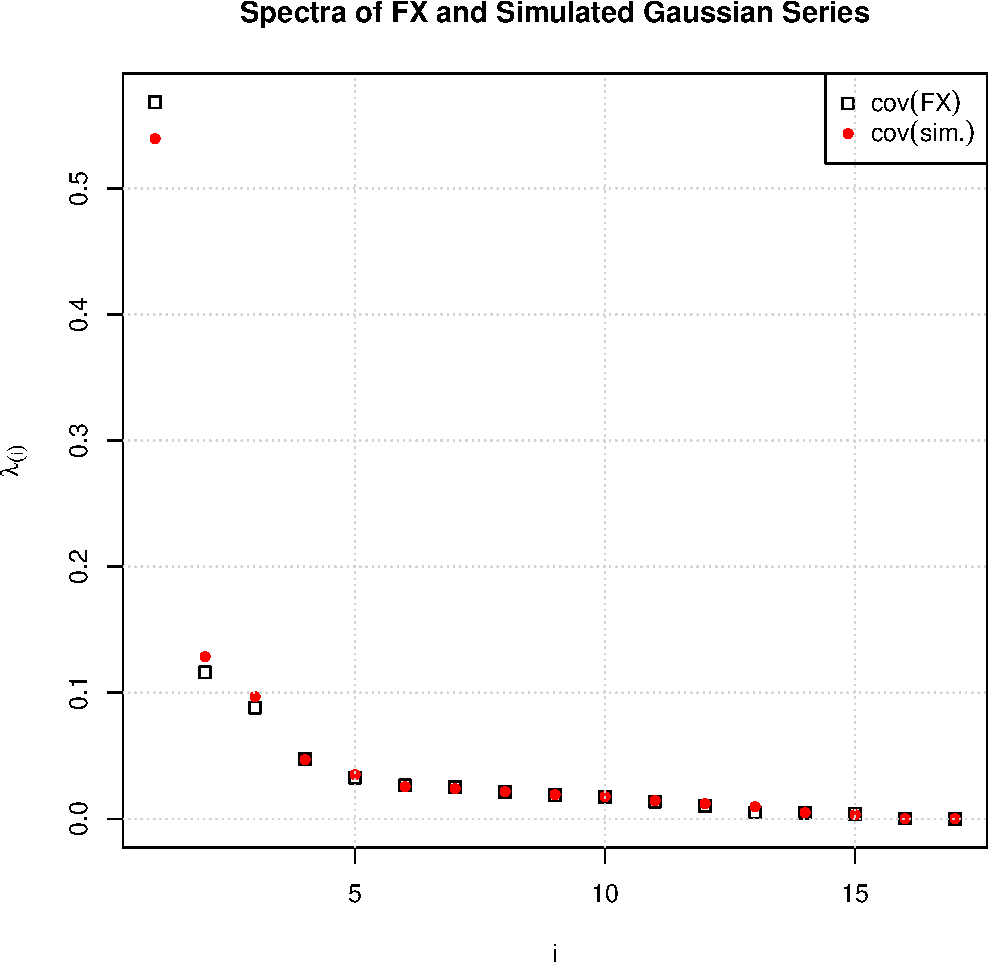
\includegraphics[width=1.0\linewidth]{Gaussian_eigenvalues.pdf}
    \caption{\scriptsize Eigenvalues of real FX series and simulated Gaussian series}
  \end{figure}
  \end{minipage}
\end{frame}

\begin{frame}
  \frametitle{Gaussian Series with the equal cov. compared with FX}
  iid. copies of $p$-variate Gaussian series with equal cov. as the FX.
  \begin{figure}[htb!]
    \centering
    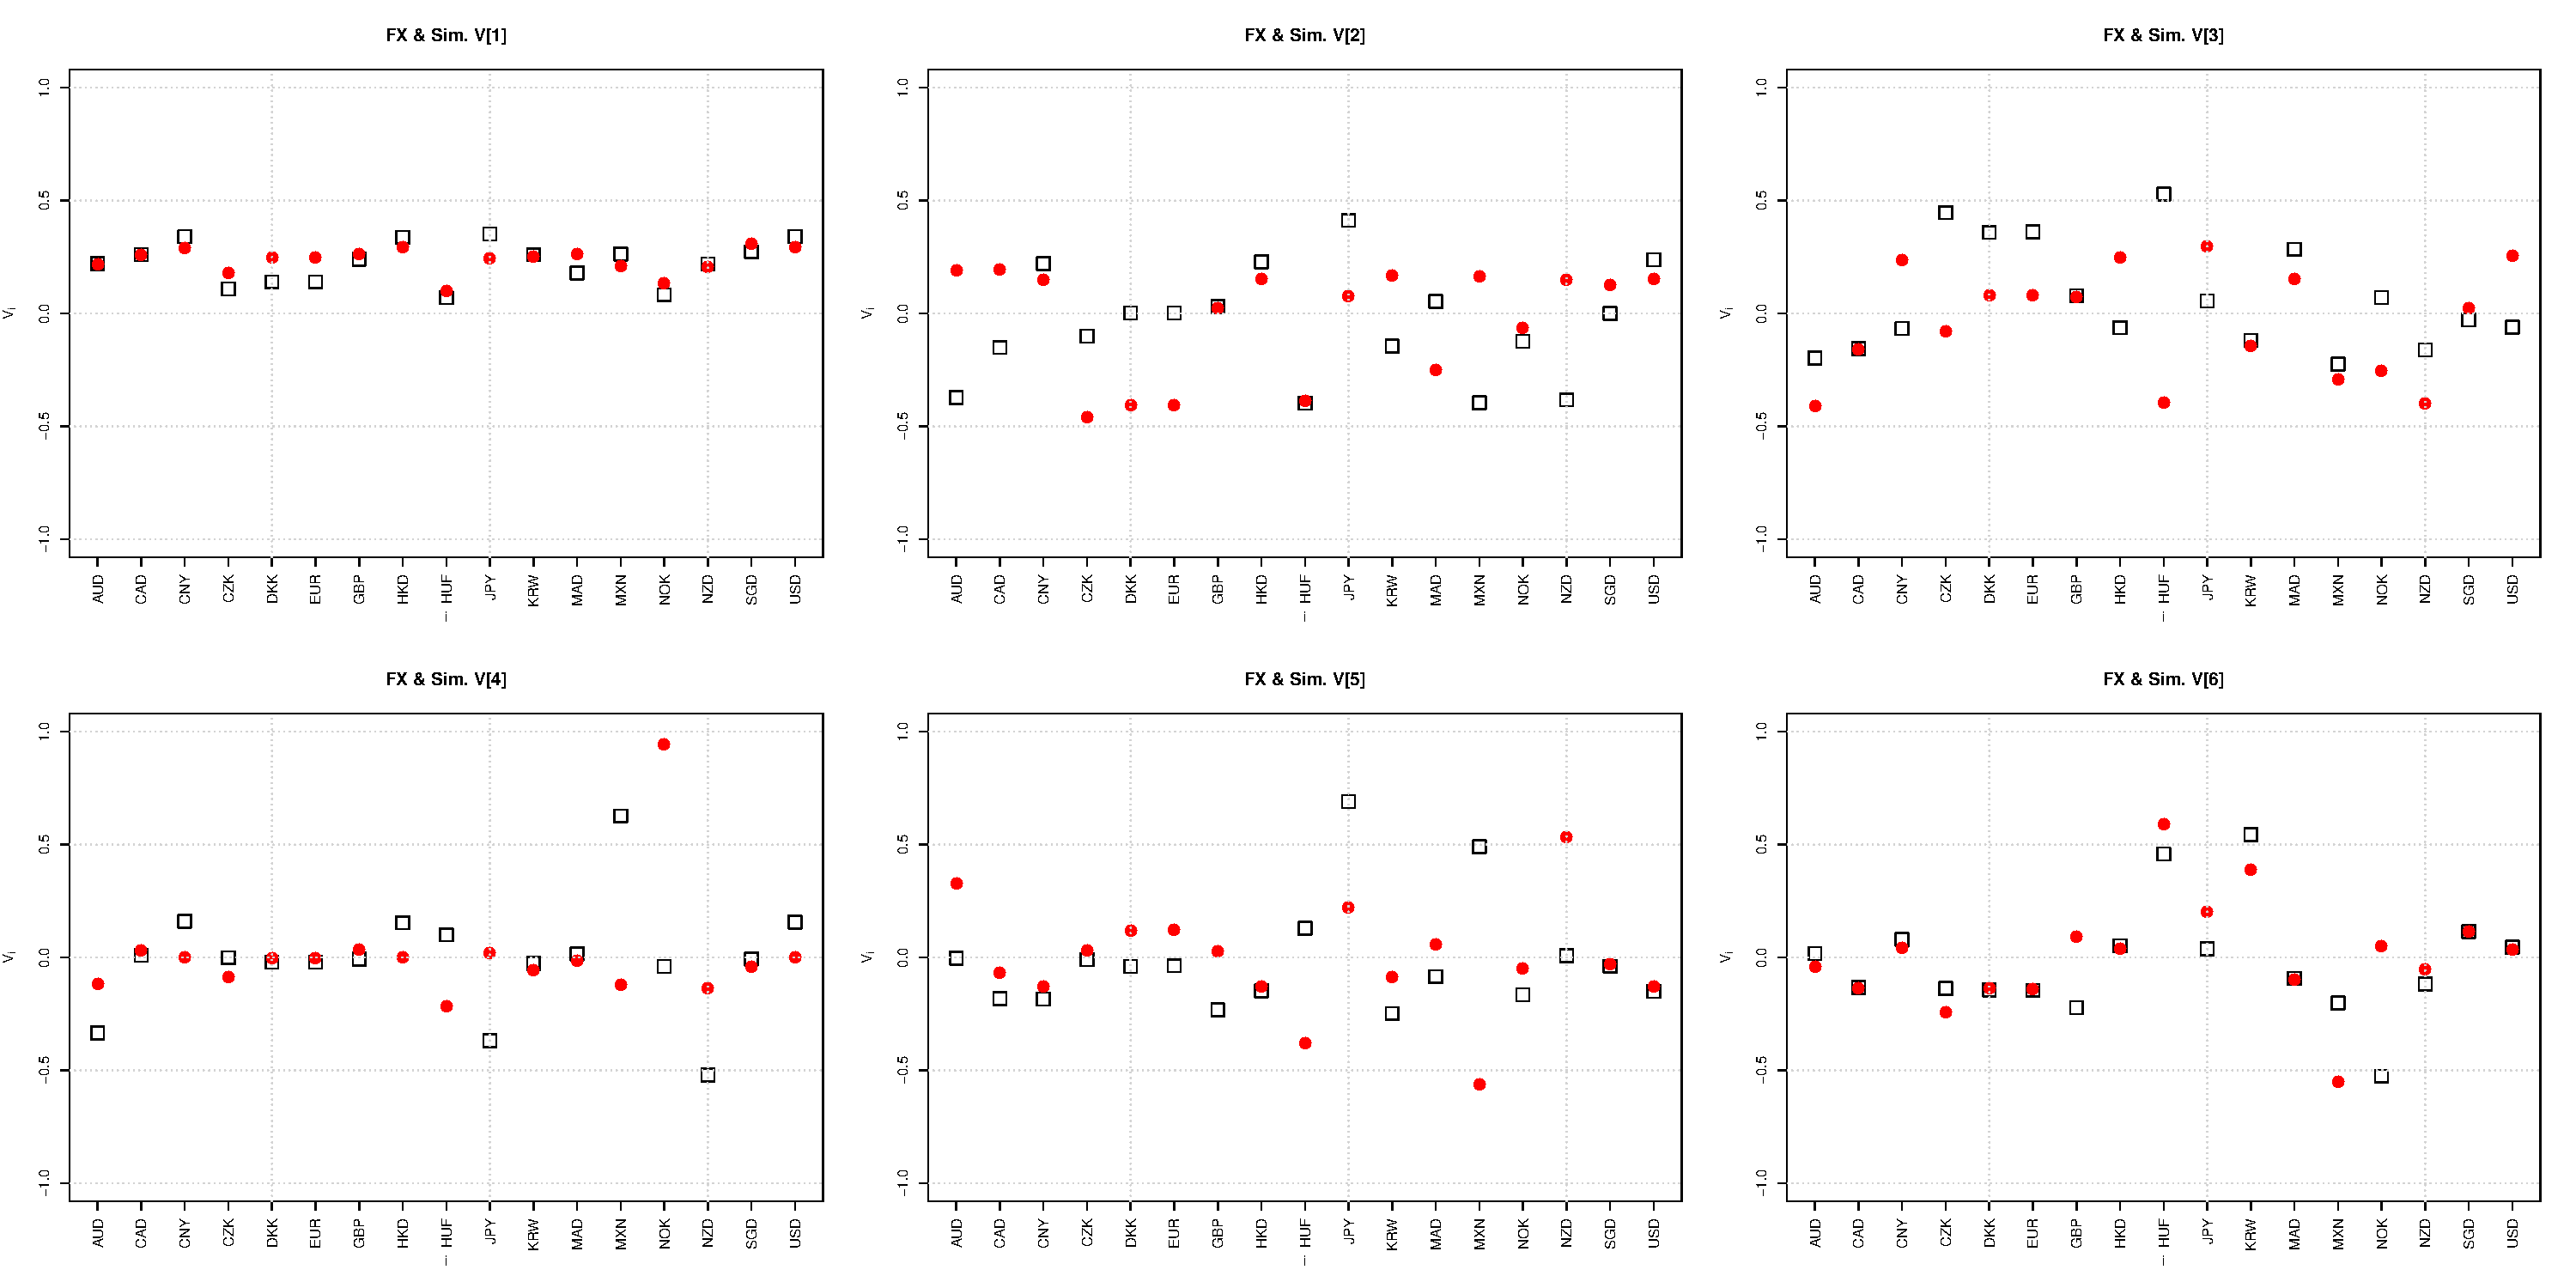
\includegraphics[width=1.0\linewidth]{Gaussian_eigenvectors.pdf}
    \caption{\scriptsize Eigenvectors of real FX series and simulated Gaussian series}
  \end{figure}
\end{frame}

\begin{frame}
  \frametitle{Stochastic Volatility Models compared with FX}
  \begin{minipage}{0.6\linewidth}
    \begin{scriptsize}
      \begin{eqnarray*}
        X_{i, t} &=& \sigma_{i, t} Z_{i,t} \\
        \ln(\sigma_{i,t})|\mathcal F_{t-1} &\sim& N(\mu + \phi(\ln(\sigma_{i,t-1})) - \mu, \zeta^2)\\
        Z_{i, t} &\bot& \ln(\sigma_{i,t})
      \end{eqnarray*}
      $\cov(\vec Z)$ \underline{same as observations}.
    \end{scriptsize}
  \end{minipage}\hfill
  \begin{minipage}{0.4\linewidth}
    \begin{figure}[htb!]
      \centering
      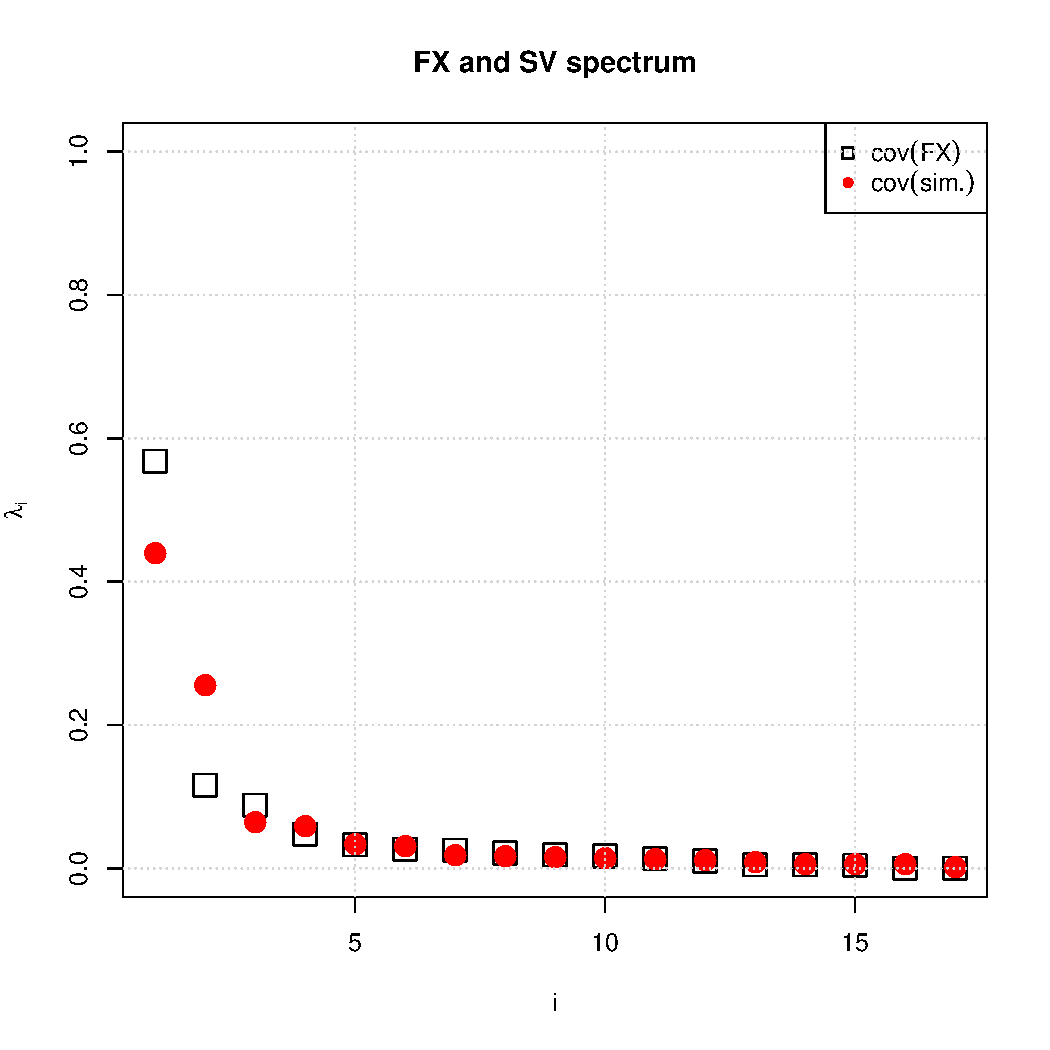
\includegraphics[width=1.0\linewidth]{FX_sv_eigenvalues.pdf}
      \caption{\scriptsize Eigenvalues of real and simulated SV series}
    \end{figure}
  \end{minipage}
\end{frame}

\begin{frame}
  \frametitle{Stochastic Volatility Models compared with FX}
  \begin{figure}[htb!]
    \centering
    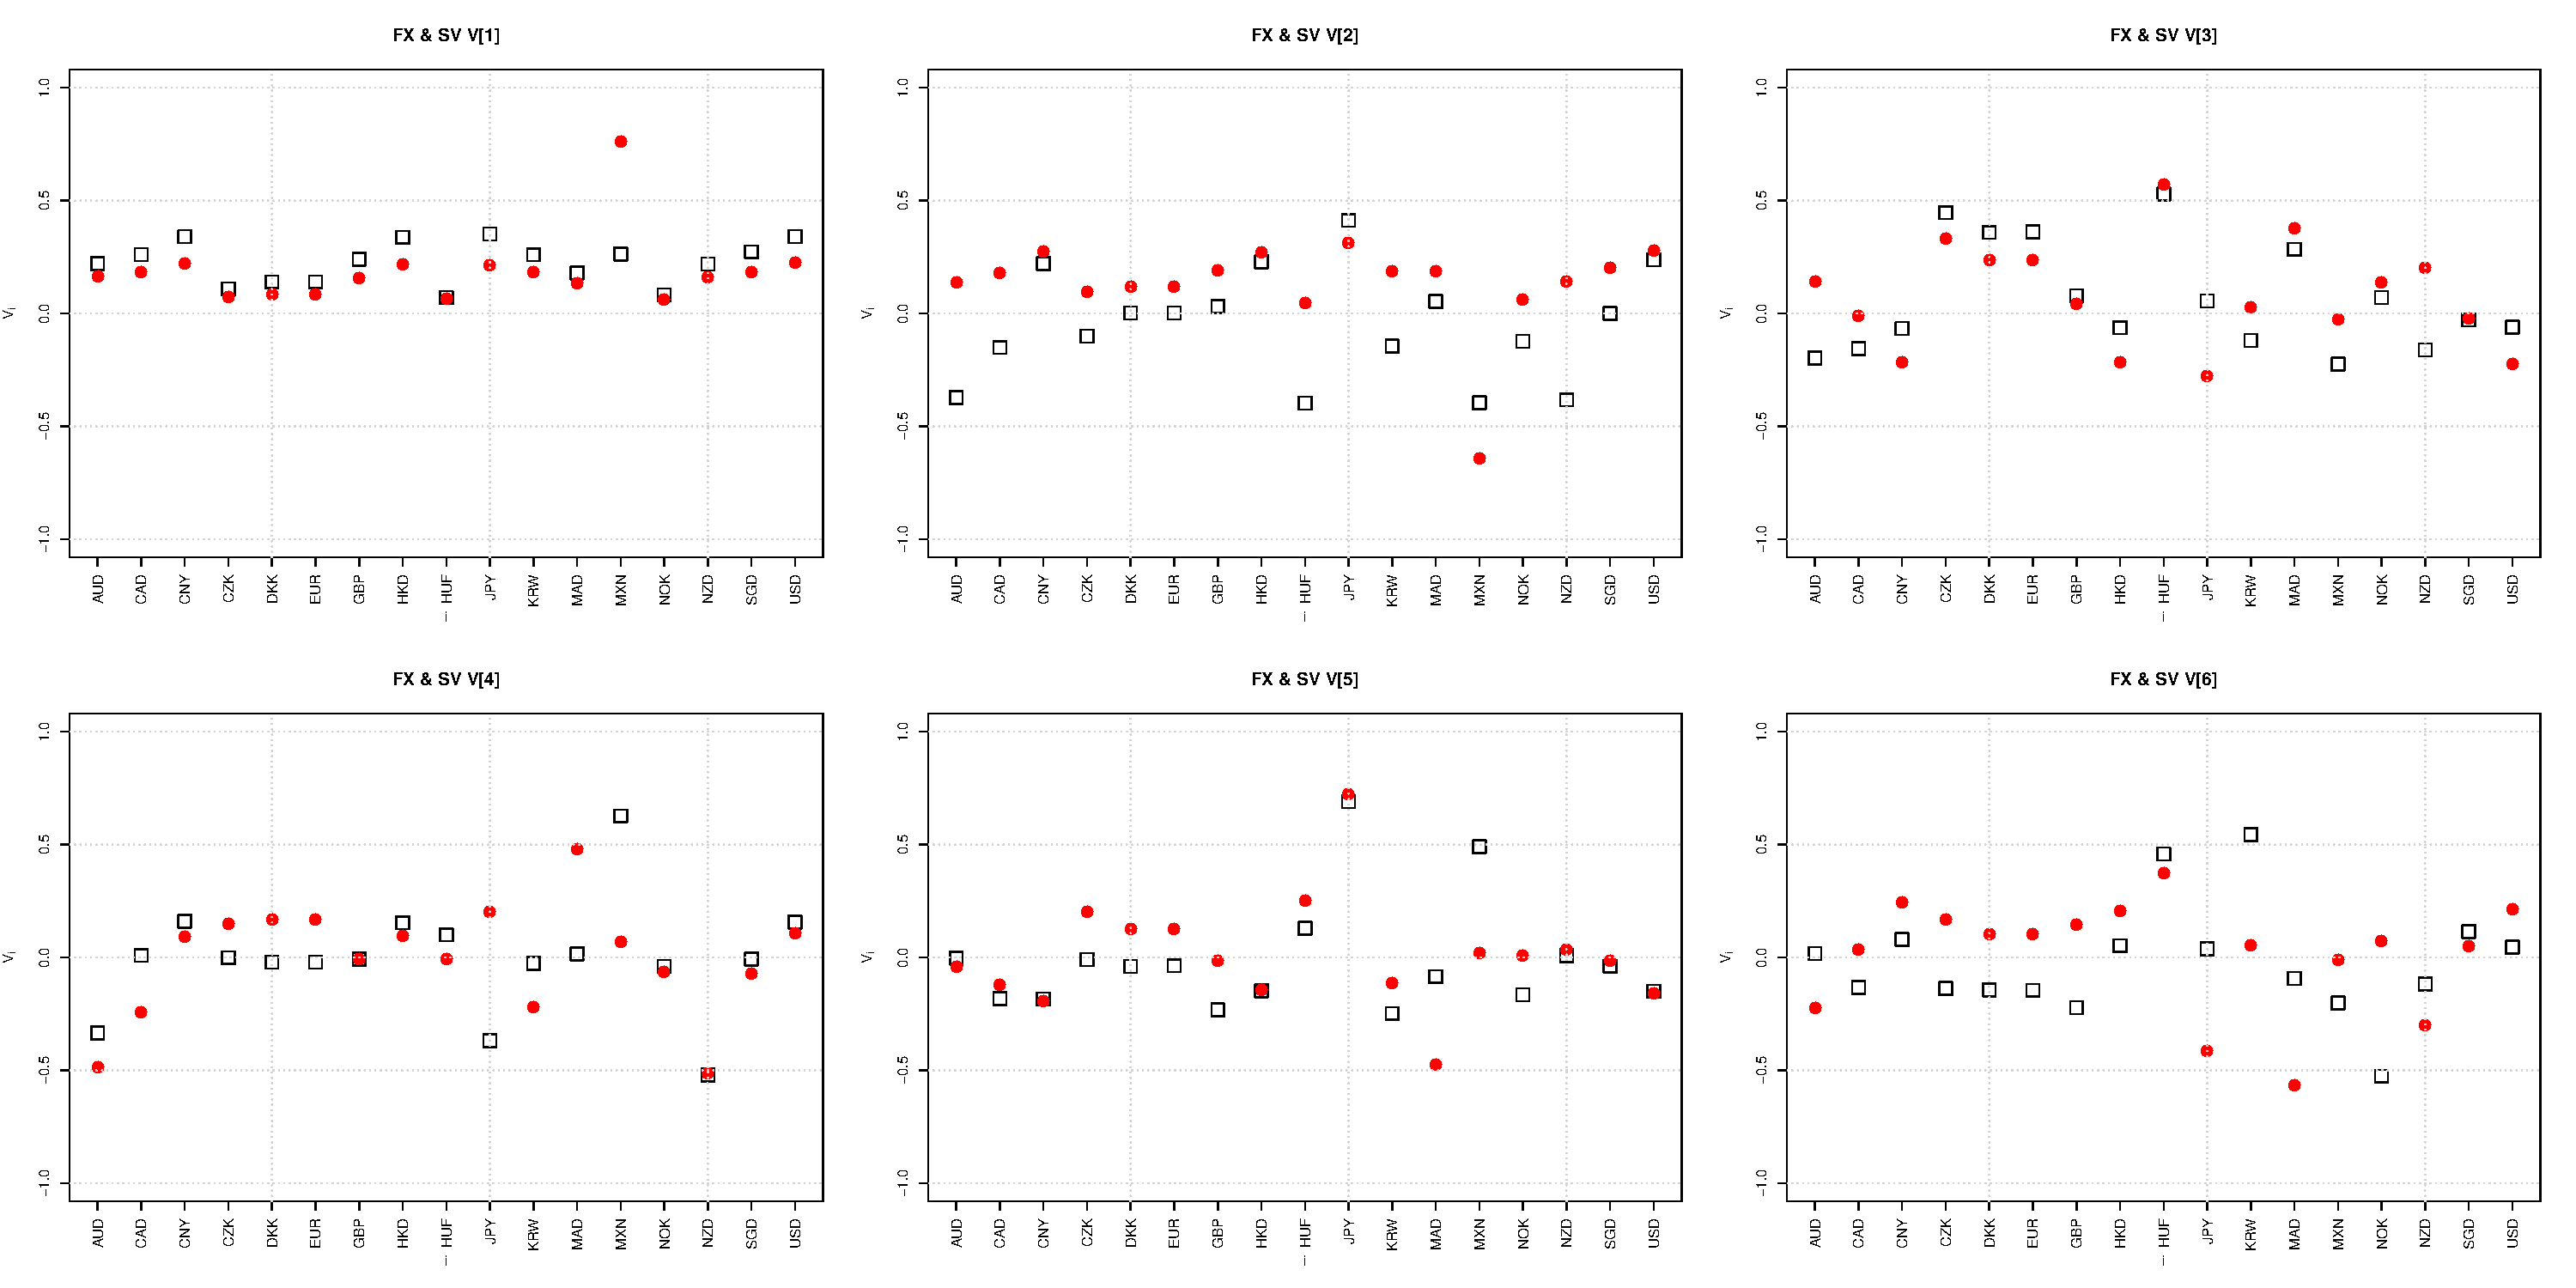
\includegraphics[width=1.0\linewidth]{FX_sv_eigenvectors.pdf}
    \caption{\scriptsize Eigenvectors of real and simulated SV series}
  \end{figure}
\end{frame}

\begin{frame}
  \frametitle{Orthogonal Combination of GARCH compared with FX}
  \begin{minipage}{0.6\linewidth}
    \begin{scriptsize}
      \begin{eqnarray*}
        X_{i, t} &=& \sum_{k=1}^N C_{i,k} Y_{k, t} + \epsilon_{i, t} \\
        Y_{k, t} &\sim& \text{GARCH}(1,1) \\
        Y_{i, t} &\bot& Y_{j, t} \quad i \neq j\\
        \epsilon_{i,t} &\sim& N(0, \sigma_i^2)
      \end{eqnarray*}
      \underline{N=8 shown in the plot}
    \end{scriptsize}
  \end{minipage}\hfill
  \begin{minipage}{0.4\linewidth}
    \begin{figure}[htb!]
      \centering
      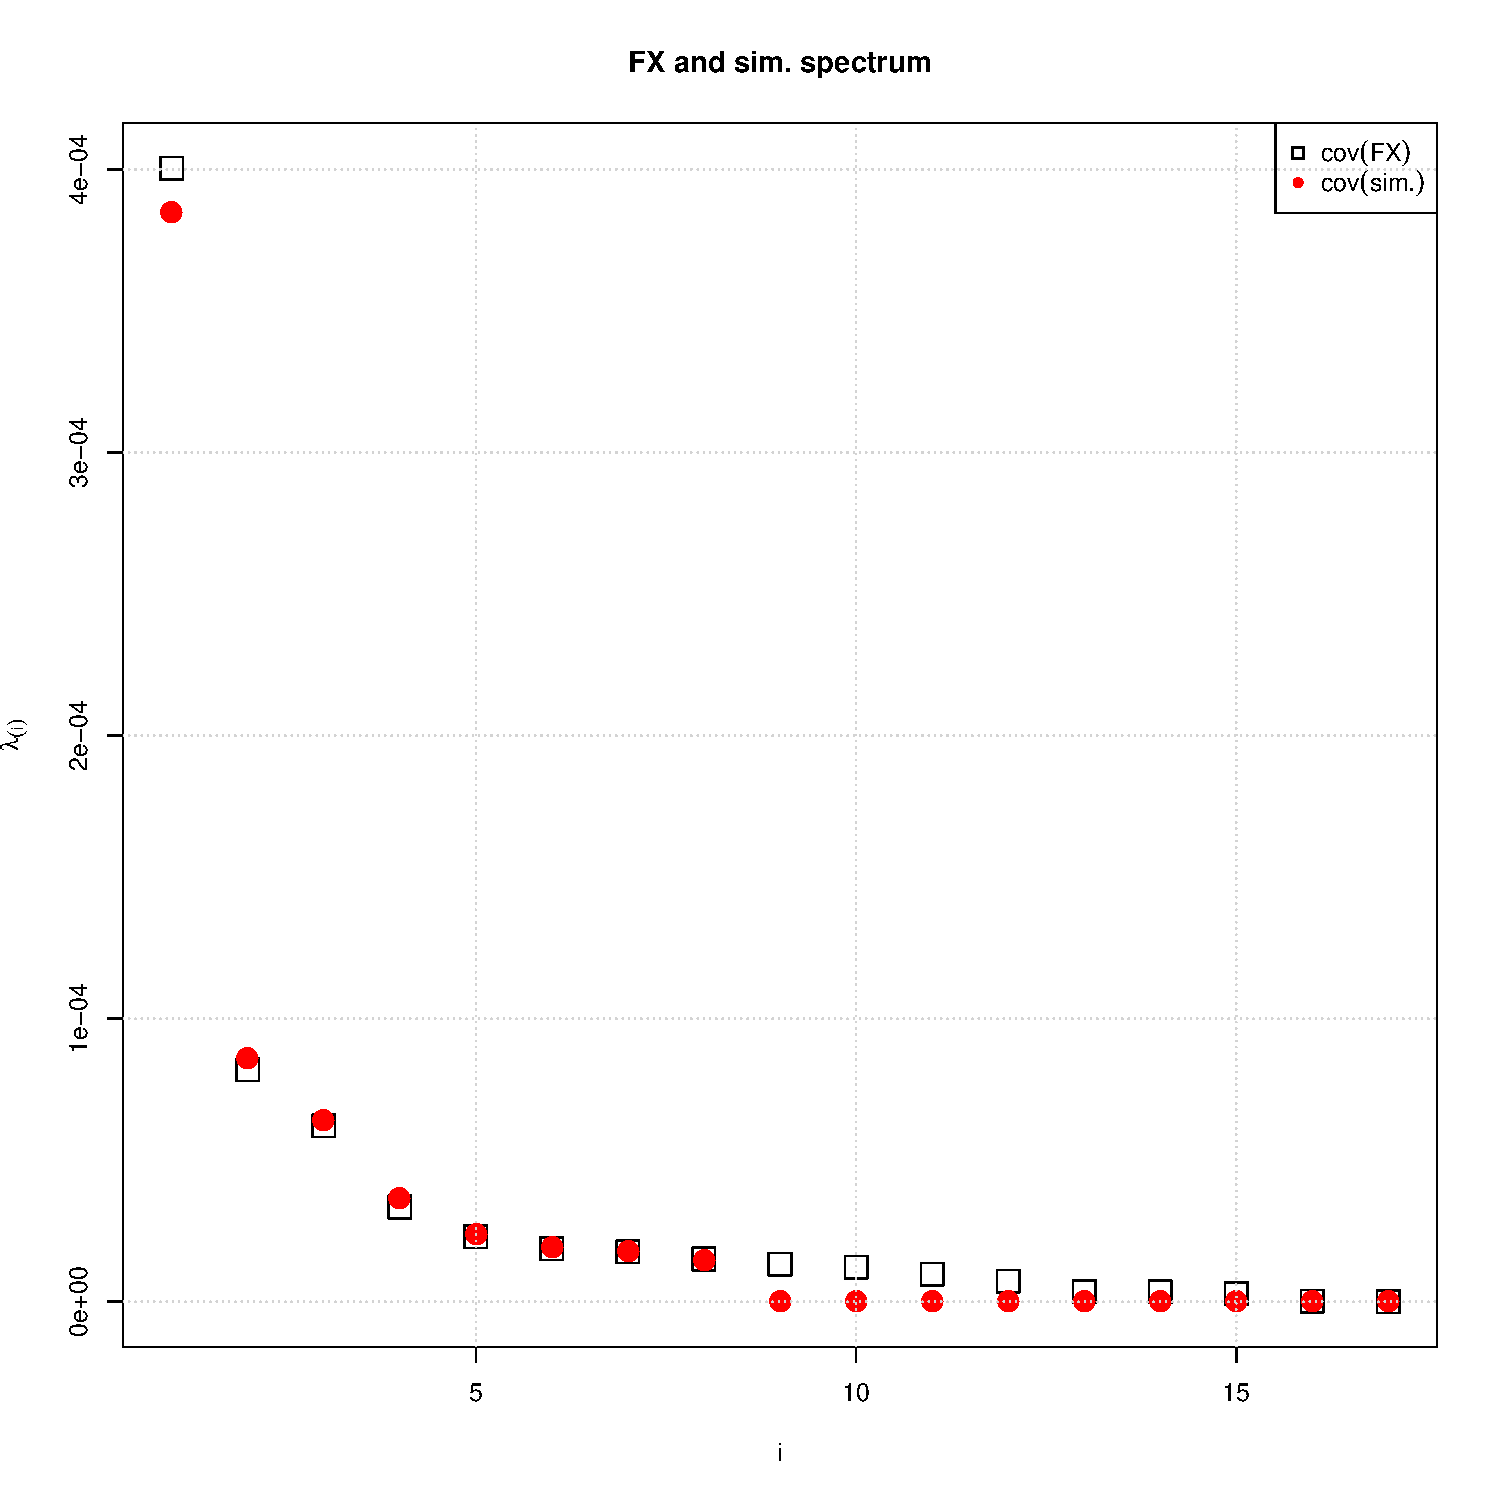
\includegraphics[width=1.0\linewidth]{FX_OGARCH_eigenvalues.pdf}
      \caption{\scriptsize Eigenvalues of real and simulated OGARCH series}
    \end{figure}
  \end{minipage}
\end{frame}

\begin{frame}
  \frametitle{Orthogonal Combination of GARCH compared with FX}
  \begin{figure}[htb!]
    \centering
    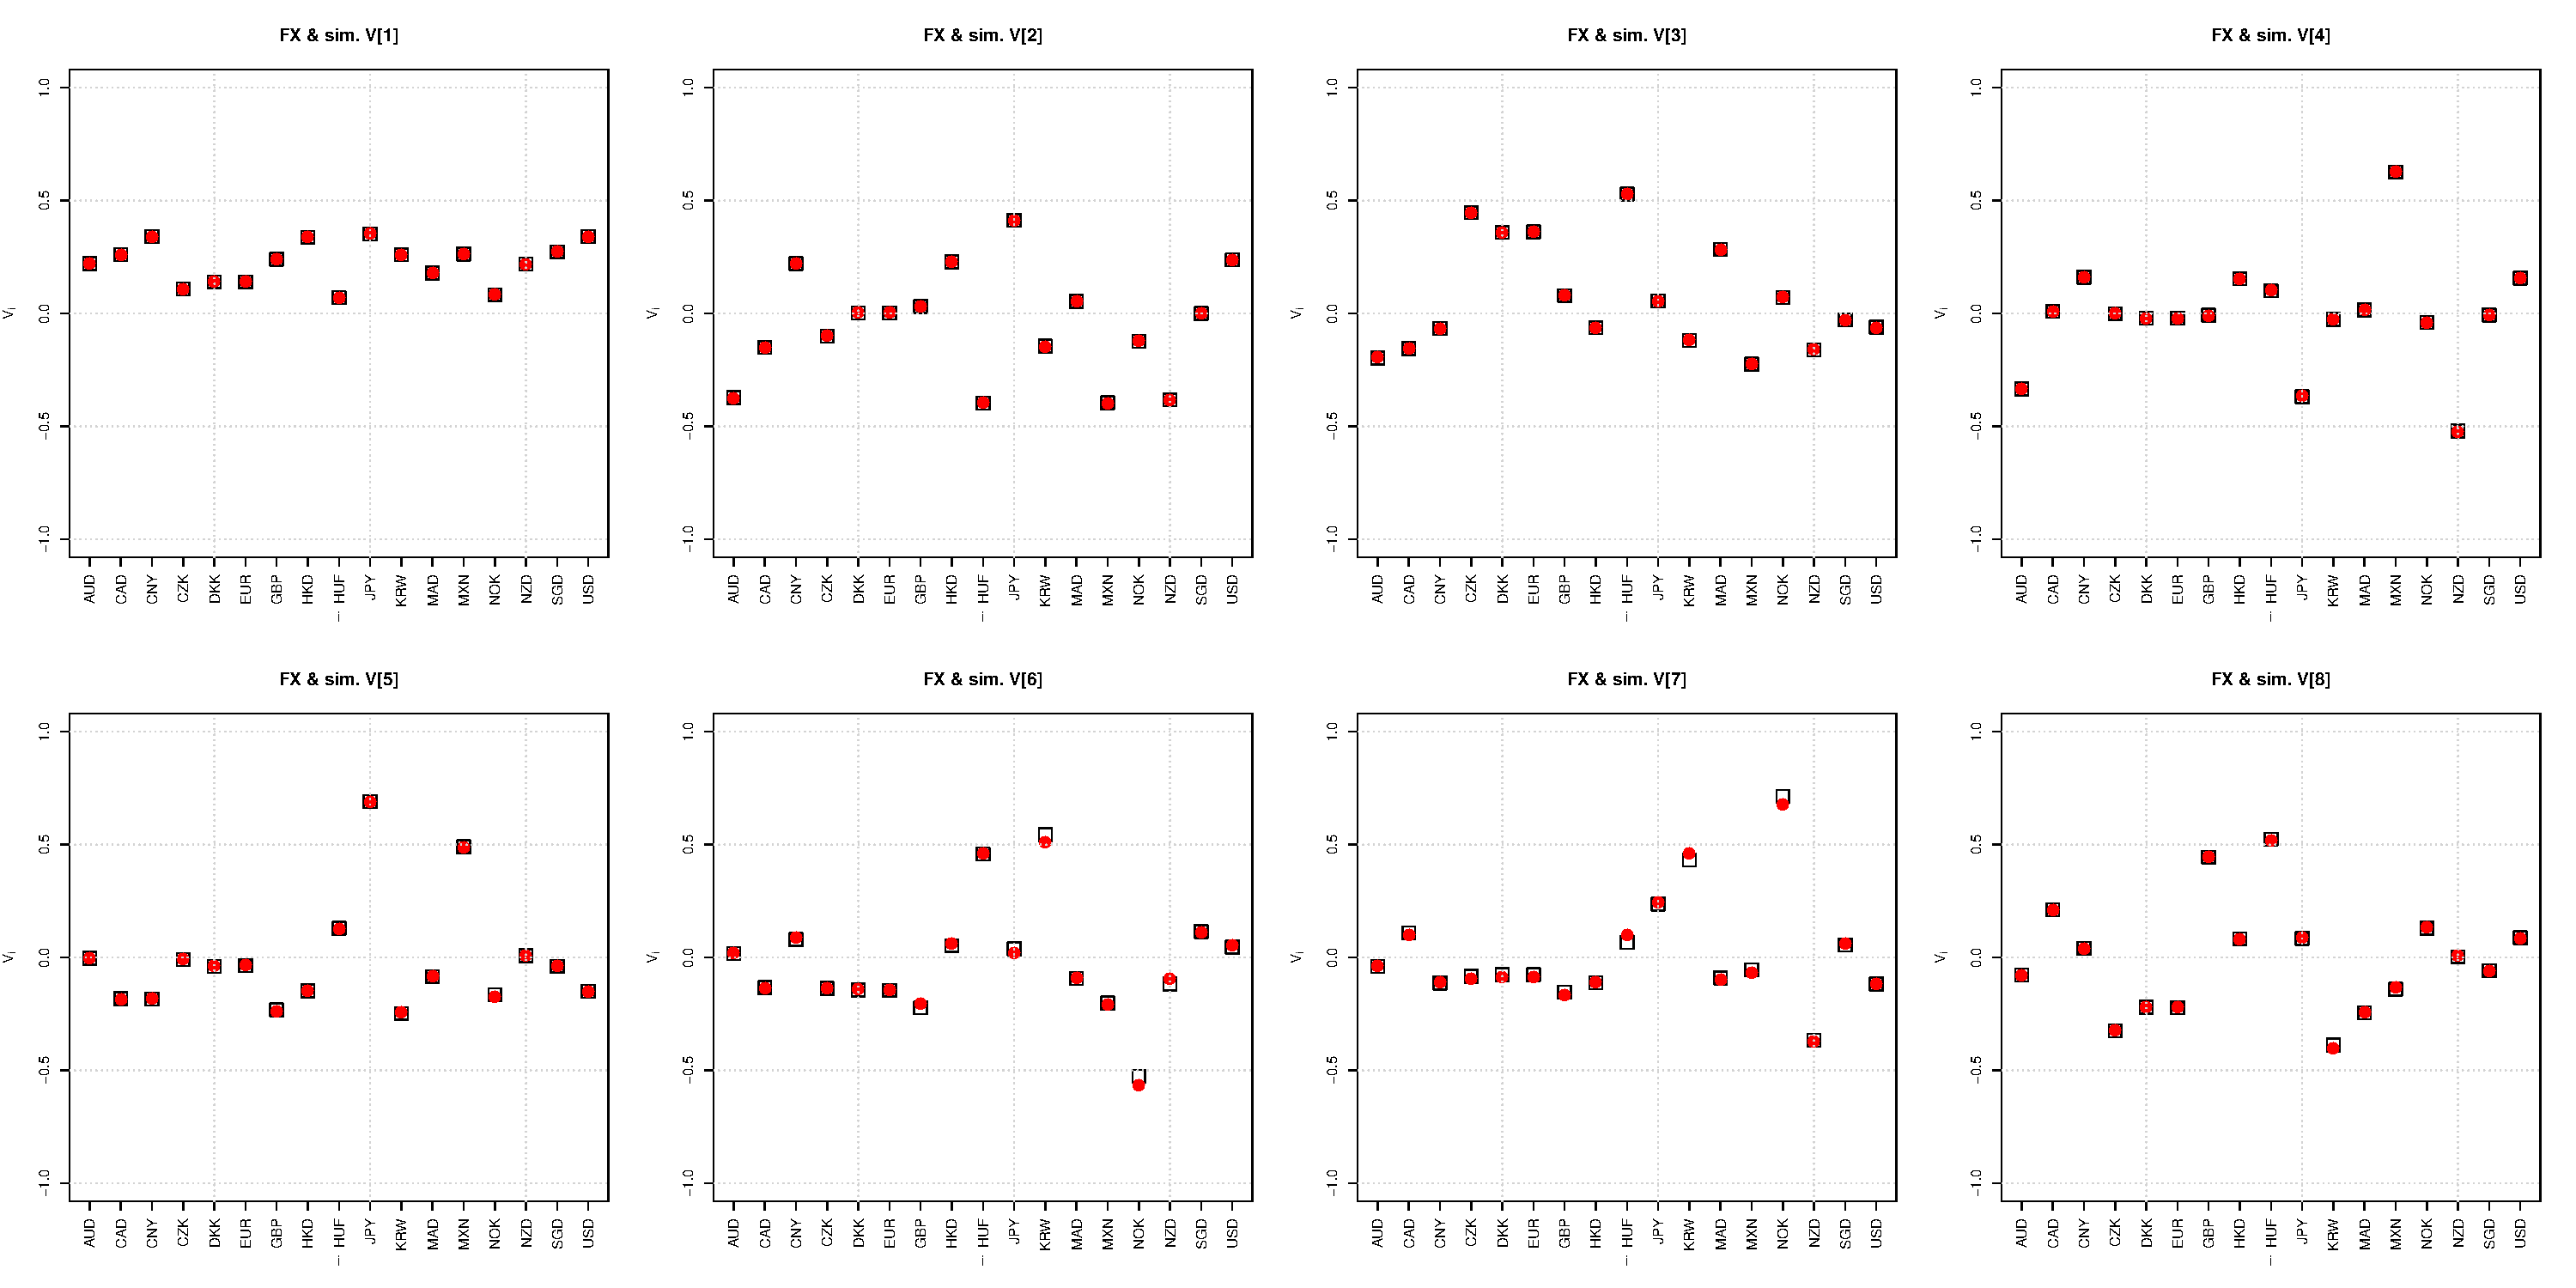
\includegraphics[scale=0.2]{FX_OGARCH_eigenvectors.pdf}
    \caption{\scriptsize Eigenvectors of real and simulated series}
  \end{figure}
\end{frame}

\begin{frame}
  \frametitle{GARCH with correlated innovations compared with FX}
  \begin{figure}[htb!]
    \centering
    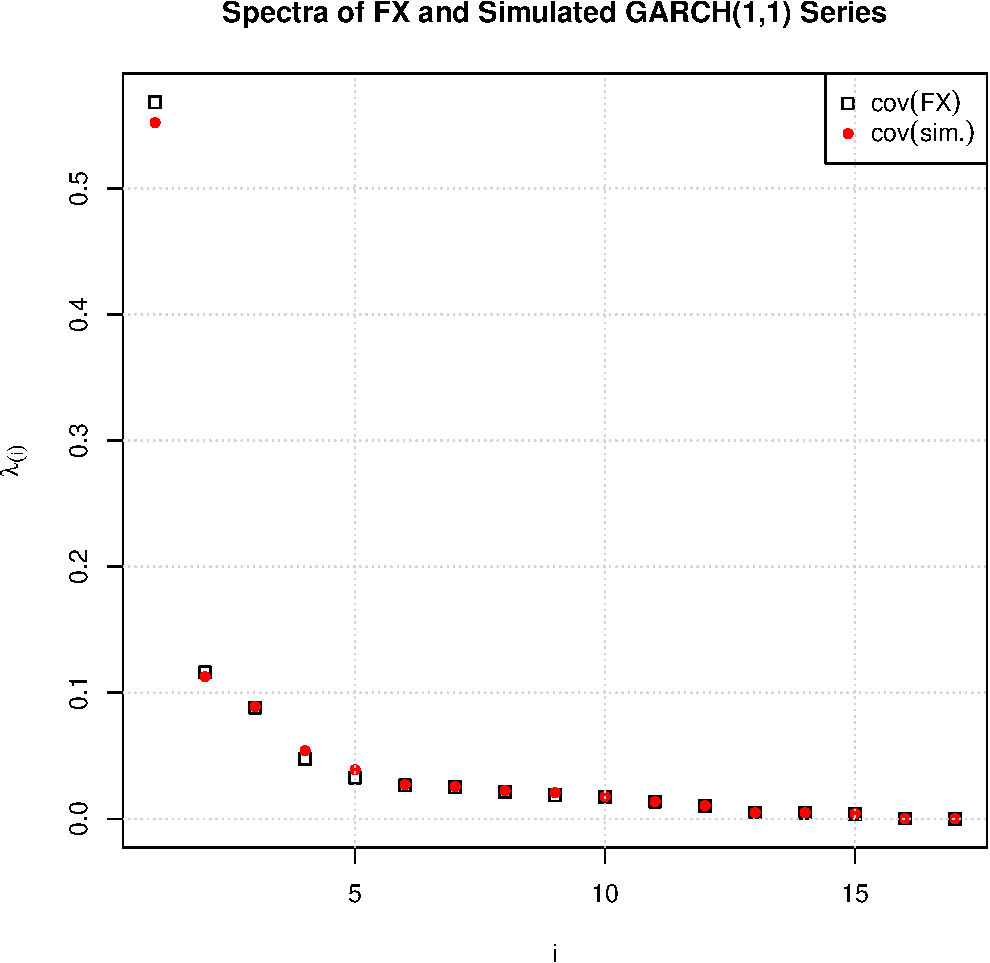
\includegraphics[scale=0.35]{FX_eigenvalues.pdf}
    \caption{\scriptsize Eigenvalues of real and simulated GARCH series}
  \end{figure}
\end{frame}

\begin{frame}
  \frametitle{GARCH with correlated innovations compared with FX}
  \begin{figure}[htb!]
    \centering
    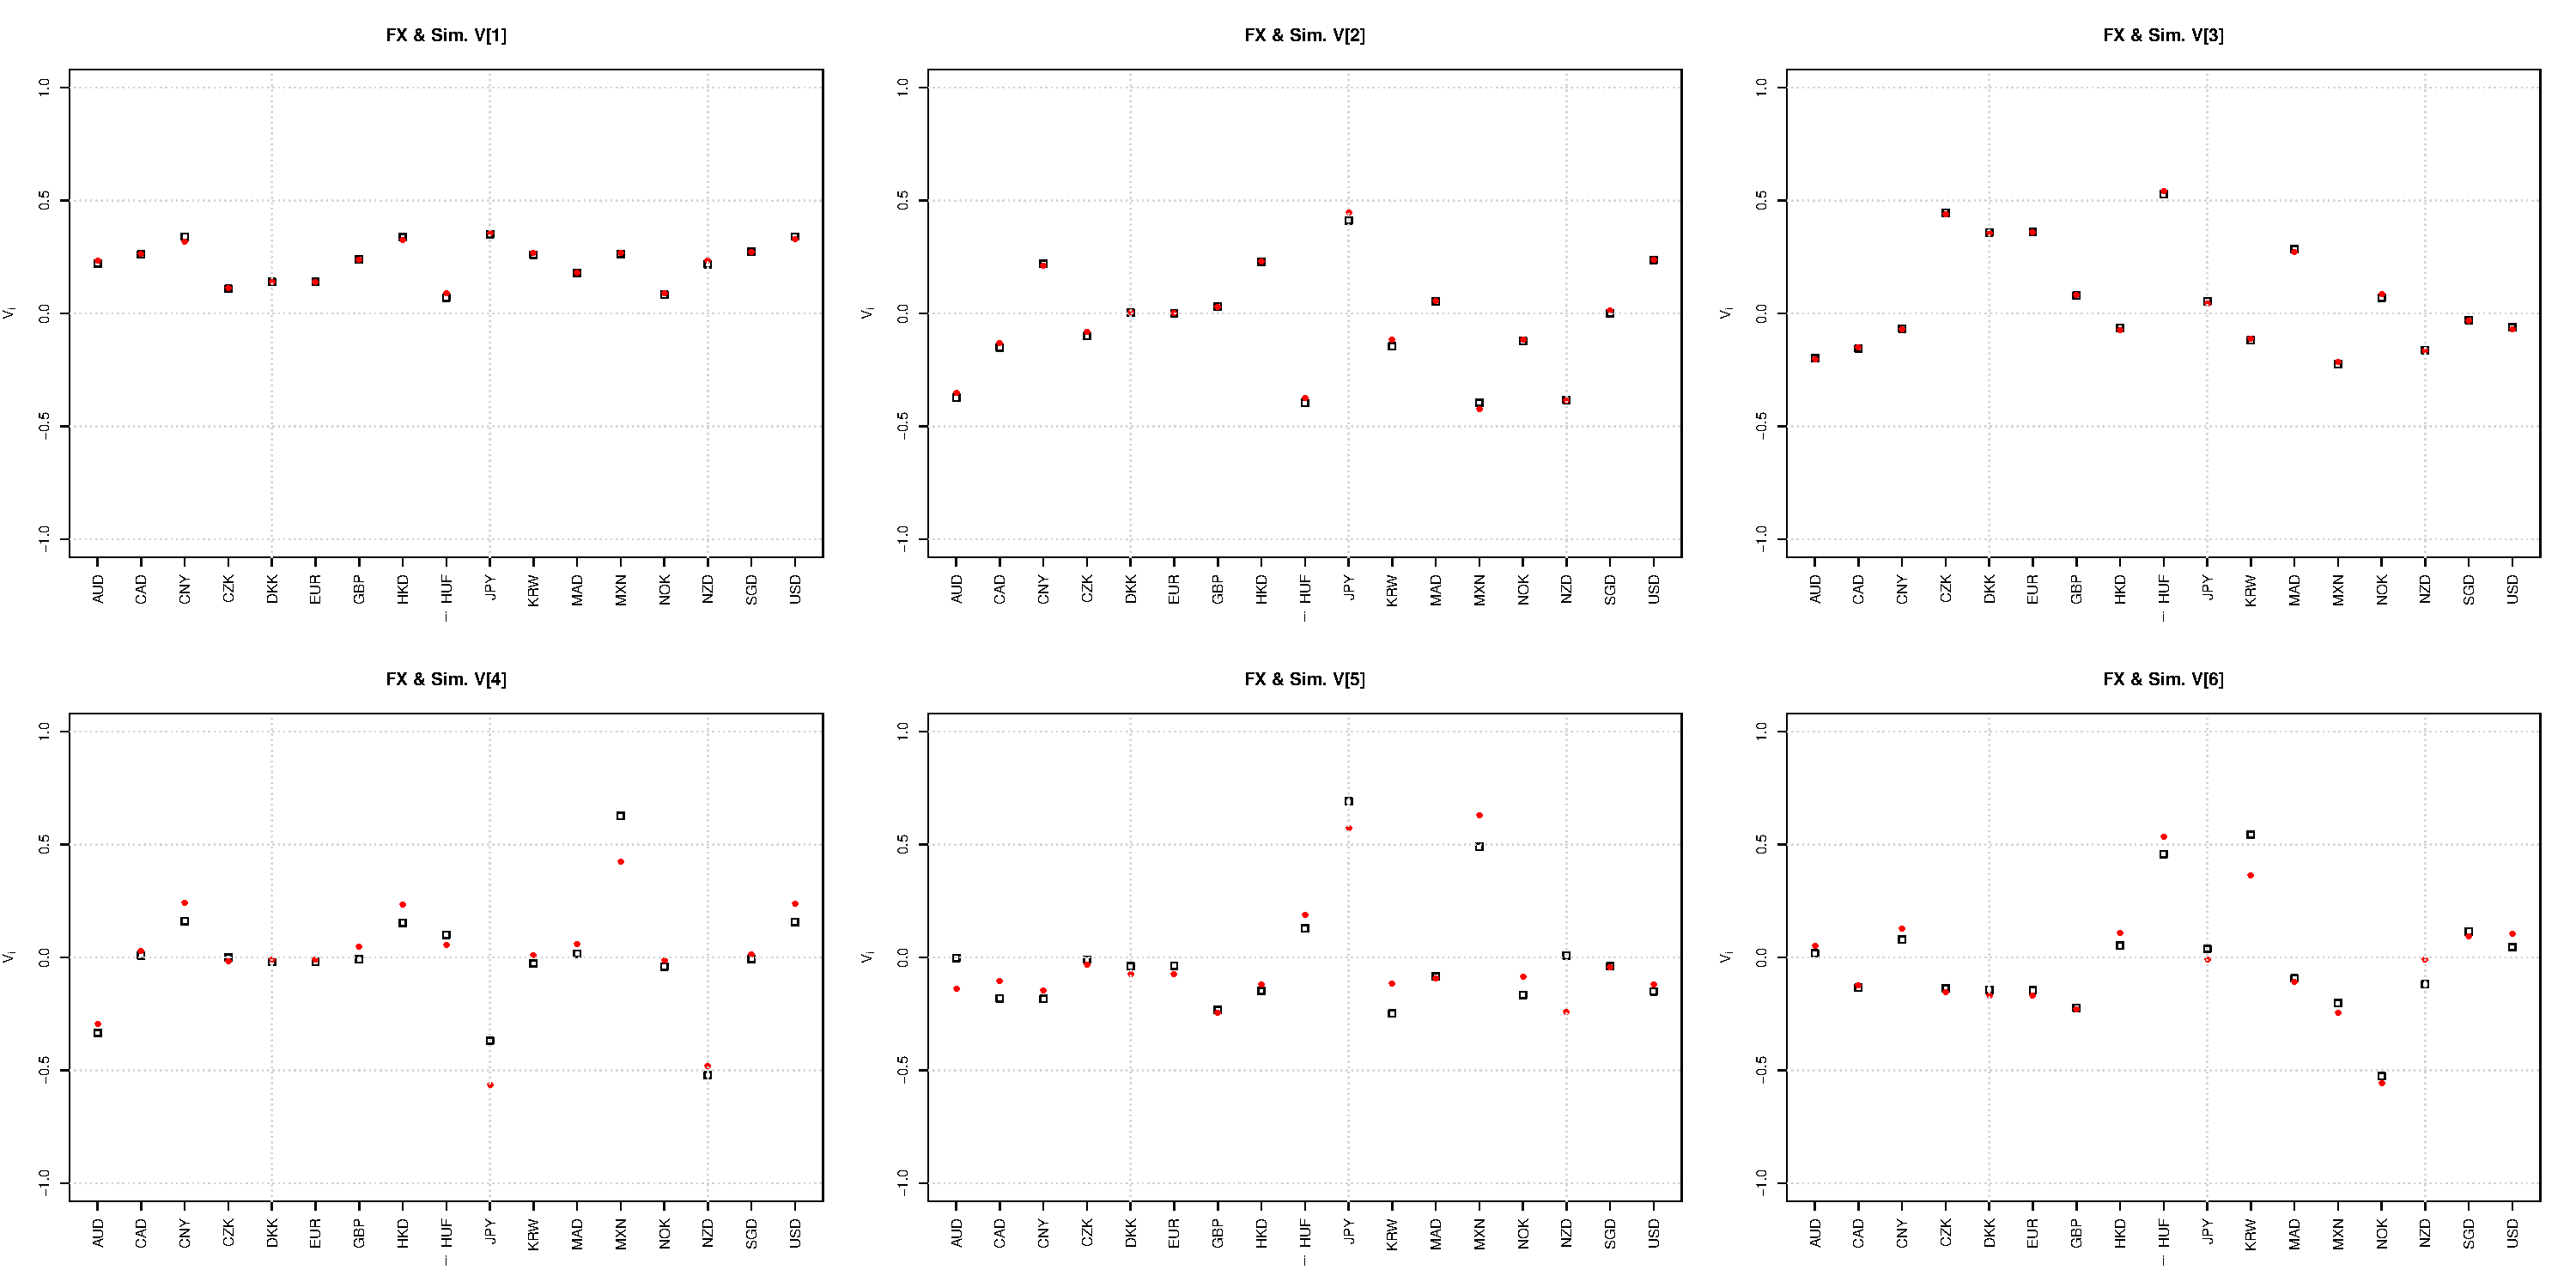
\includegraphics[scale=0.2]{FX_eigenvectors.pdf}
    \caption{\scriptsize Eigenvectors of real and simulated GARCH series}
  \end{figure}
\end{frame}

  
\subsection{Utilities}
\begin{frame}
  \frametitle{Sector of Utilities of S\&P 500}
  Daily return series of 23 companies in the S\&P 500 Utilities sector
  fitted to {\bf GARCH with correlated innovations}.
  \begin{figure}[htb!]
    \centering
    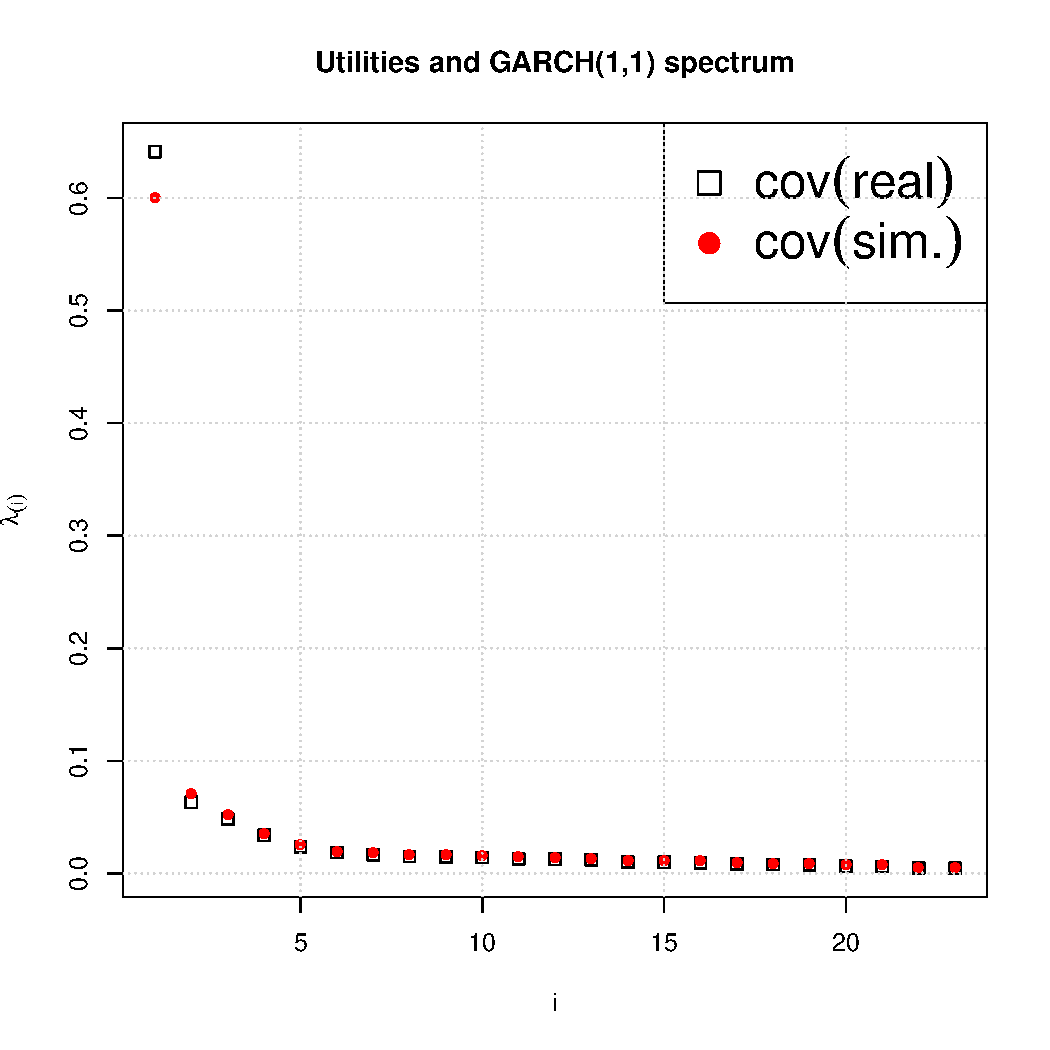
\includegraphics[scale=0.35]{Utilities_eigenvalues.pdf}
    \caption{\scriptsize Eigenvalues of real and simulated GARCH series}
  \end{figure}
\end{frame}

\begin{frame}
  \frametitle{Sector of Utilities of S\&P 500}
  Daily return series of 23 companies in the S\&P 500 Utilities sector
  fitted to {\bf GARCH with correlated innovations}.
  \begin{figure}[htb!]
    \centering
    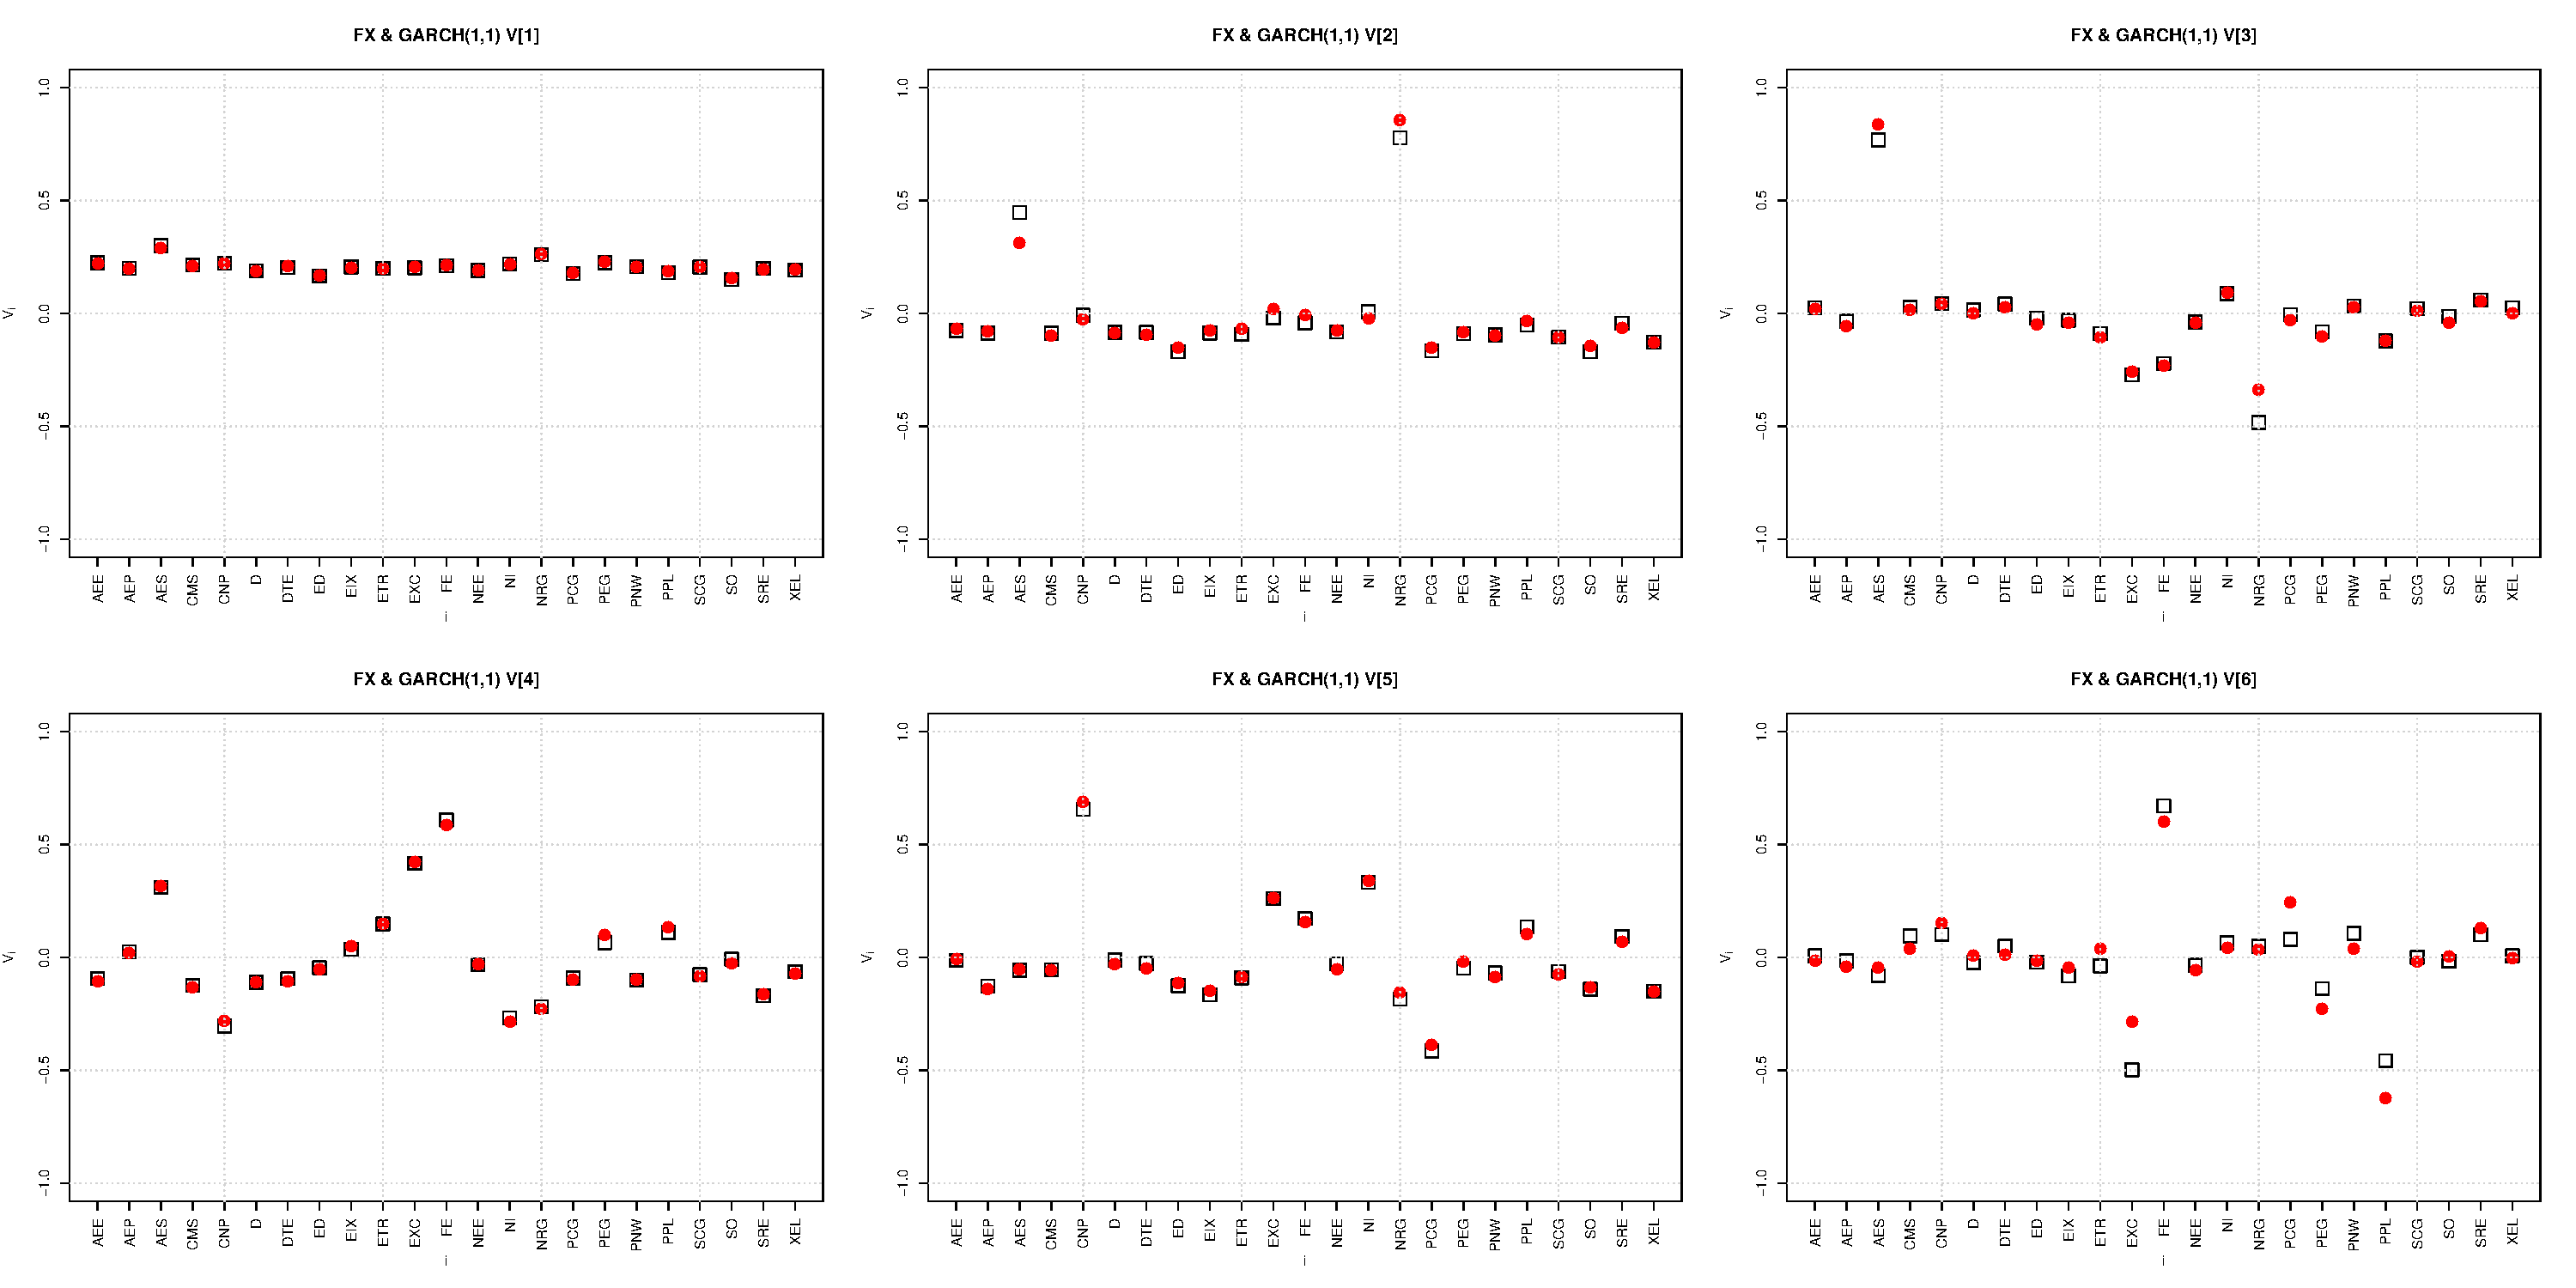
\includegraphics[width=1.0\linewidth]{Utilities_eigenvectors1.pdf}
    \caption{\scriptsize Eigenvectors of real and simulated GARCH series}
  \end{figure}
\end{frame}

\subsection{Materials}
\begin{frame}
  \frametitle{Sector of Materials of S\&P 500}
  Daily return series of 21 companies in the S\&P 500 Materials sector
  fitted to {\bf GARCH with correlated innovations}.
  \begin{figure}[htb!]
    \centering
    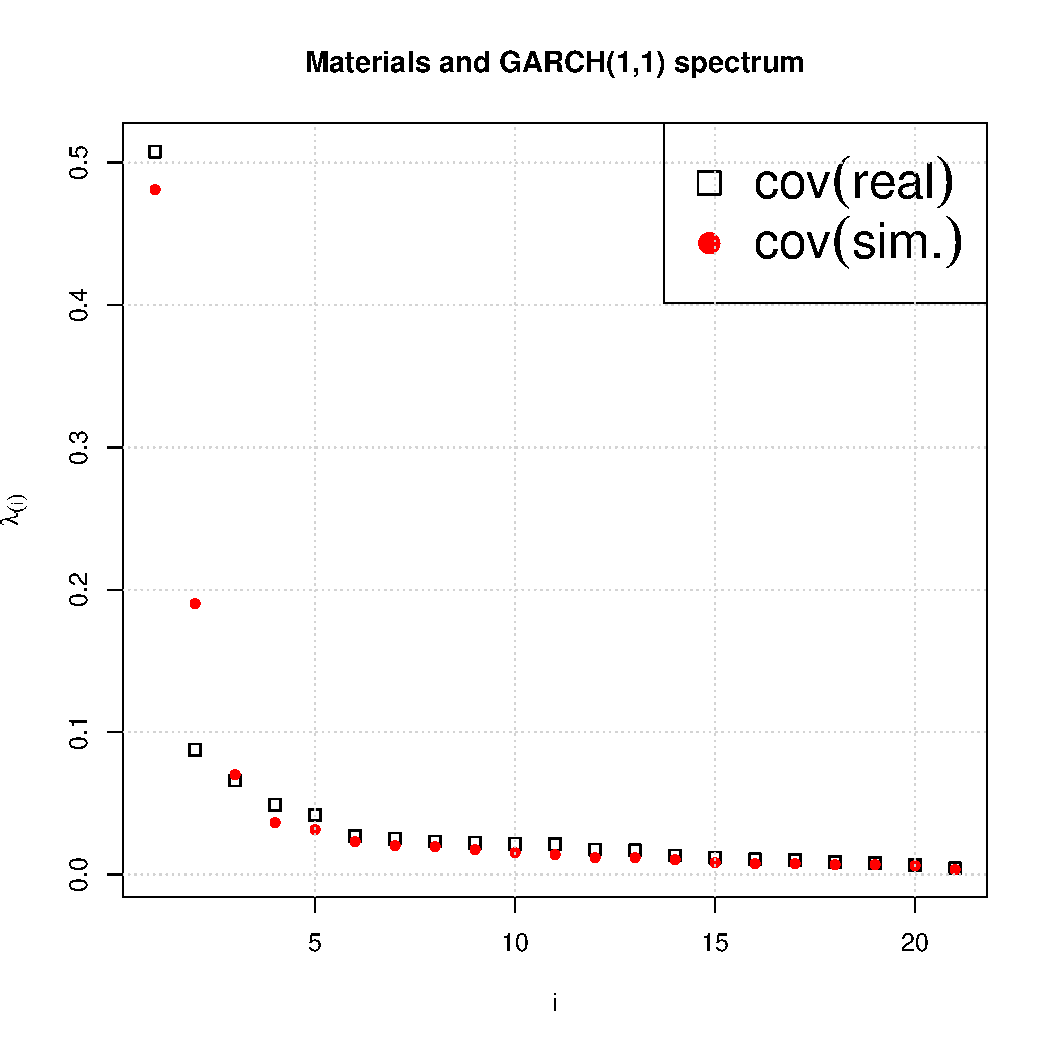
\includegraphics[scale=0.35]{Materials_eigenvalues.pdf}
    \caption{\scriptsize Eigenvalues of real and simulated GARCH series}
  \end{figure}
\end{frame}

\begin{frame}
  \frametitle{Sector of Materials of S\&P 500}
  Daily return series of 21 companies in the S\&P 500 Materials sector
  fitted to {\bf GARCH with correlated innovations}.
  \begin{figure}[htb!]
    \centering
    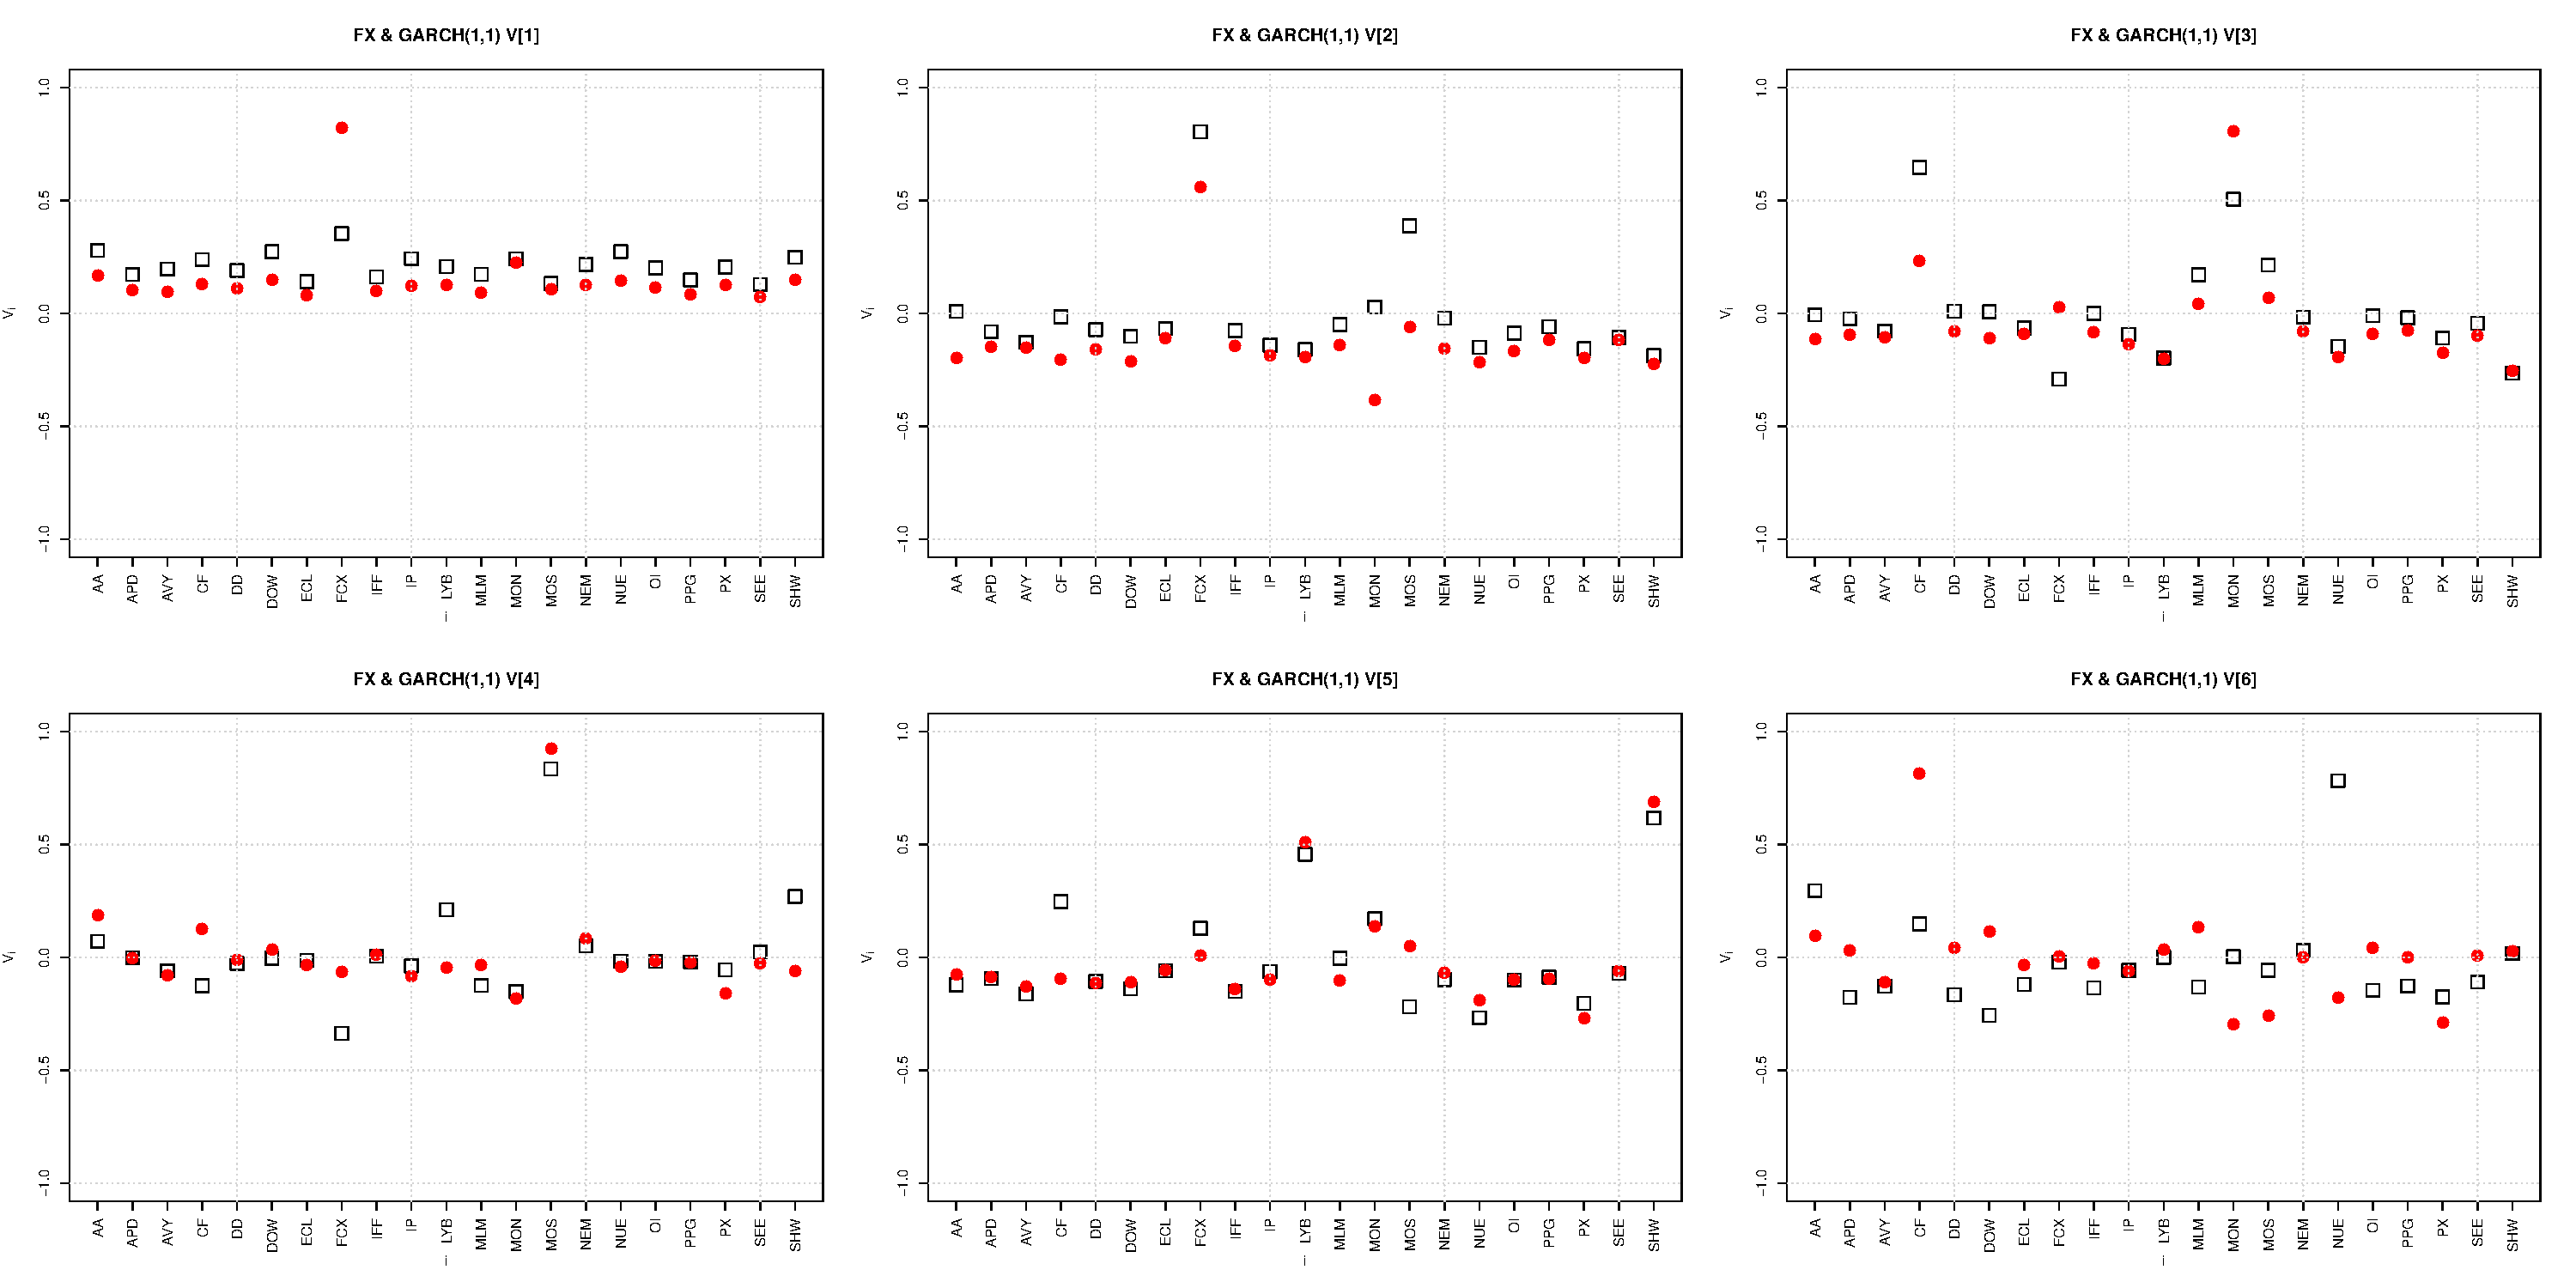
\includegraphics[width=1.0\linewidth]{Materials_eigenvectors1.pdf}
    \caption{\scriptsize Eigenvectors of real and simulated GARCH series}
  \end{figure}
\end{frame}

\subsection{Emergence of the Observed Spectrum}
\begin{frame}
  \frametitle{Regular Variation}
  \begin{minipage}[t]{0.4\linewidth}
    \textcolor[HTML]{990033}{Univariate regular variation}
    Distribution of $X$ has regularly varying tail with index $\alpha$:
    \[
    \lim_{u \to \infty}
    {
      \P(X > t u)
      \over
      \P(X > u)
    } = t^{-\alpha}
    \]
  \end{minipage}\hfill
  \begin{minipage}[t]{0.55\linewidth}
    \textcolor[HTML]{990033}{Joint regular variation}    
    Joint distribution of $\vec X = (X_1, X_2, ..., X_p)$ regular
    varying with tail index $\alpha$:
    \[
    \lim_{u \to \infty}
    {
      \P(u^{-1} X \in \cdot)
      \over
      \P(|X|>u)
    } = \mu(\cdot)
    \]
    $\mu$: A non-null Radon measure on $(\mathbb R^d \setminus \{\vec
    0\}) \cup \{-\infty, \infty\}$:
    \[
      \mu(t \mathcal C) =
      t^{-\alpha} \mu(\mathcal C)
    \]
    for all $t > 0$ and $\mu$-continuity set $\mathcal C$,
    i.e. $\mu(\partial \mathcal C) = 0$. Equivalently:
    \[
    {
      \P(|\vec X| > t u, \vec{\tilde X} \in \cdot)
      \over
      \P(|\vec X| > u)
    } \overset{w}{\to} t^{-\alpha} P_\Theta(\cdot)
    \]
  \end{minipage}
\end{frame}

\begin{frame}
  \frametitle{Emergence of the Observed Spectrum}
  Conjecture: Joint regular variation of the entries of the covariance
  matrix leads to the observed spectral pattern.
  \begin{itemize}
  \item $(X_{1,t}, ..., X_{p,t})$ jointly regularly varying with
    different indices $\kappa_1, ..., \kappa_p$.
  \item $(X_{1,t}^2, ..., X_{p,t}^2, \{X_{i,t} X_{j,t}\}_{1 \leq i < j
      \leq p})$ jointly regularly varying with different indices
  \item Tail index of $X_{i,t} X_{j,t}$ ($\kappa_{i,j}$) possibly
    smaller than $\min\{\kappa_i, \kappa_j\}$.
  \end{itemize}
  Want to find dominant components, say $X_{i,t}^2, X_{j,t}^2,
  X_{i,t} X_{j,t}, X_{k,t} X_{l,t}$ that are regularly varying with
  the smallest tail index.
\end{frame}

\begin{frame}
  \frametitle{The Tail index $\kappa_i$}
  Consider the tail indices of the entries of the covariance matrix C:
  For the diagonal entries
    \begin{eqnarray*}
      C_{i, i} &=& \sum_{t=1}^n X_{i, t}^2 \\
               &=& \sum_{t=1}^n Z_{i, t}^2 \sigma_{i, t}^2 \\
    \end{eqnarray*}
    $Z_{i, t}^2$ is light tailed, so $Z_{i, t}^2 \sigma_{i, t}^2$ has
    the same tail index as $\sigma_{i, t}^2$.
    \[
    \sigma_{i, t}^2 = \omega + (\alpha_i Z_{i,t}^2 + \beta_i)\sigma_{i,t-1}^2
    \]
    So by Goldie-Kesten theorem, $\kappa_i$ is given by
    \[
    \E (\alpha_i Z^2 + \beta_i)^{\kappa_i} = 1
    \]
    where $Z \sim N(0, 1)$.
  \end{frame}

  \begin{frame}
  \frametitle{The Tail index $\kappa_{i,j}$}
    For the non-diagonal entries
    \begin{eqnarray*}
      C_{i, j} &=& \sum_{t=1}^n X_{i, t} X_{j, t} \\
      &=& \sum_{t=1}^n Z_{i, t} Z_{j, t} \sigma_{i, t} \sigma_{j, t}
    \end{eqnarray*}

    \begin{tiny}
      \begin{eqnarray*}
        \begin{pmatrix}
          \sigma_{i,t}^2 \sigma_{j,t}^2 \\
          \sigma_{i,t}^2 \\
          \sigma_{j,t}^2
        \end{pmatrix}
        &=&
        \begin{pmatrix}
          (\alpha_i Z_{i,t}^2 + \beta_i) (\alpha_j Z_{i,t}^2 + \beta_j) & \omega_j & \omega_i \\
          0 & \alpha_i Z_{i,t}^2 + \beta_i & 0 \\
          0 & 0 & \alpha_j Z_{i,t}^2 + \beta_j
        \end{pmatrix}
        \begin{pmatrix}
          \sigma_{i,t-1}^2 \sigma_{j,t-1}^2 \\
          \sigma_{i,t-1}^2 \\
          \sigma_{j,t-1}^2
        \end{pmatrix} +
        \begin{pmatrix}
          \omega_i \omega_j\\
          \omega_i \\
          \omega_j
        \end{pmatrix}
      \end{eqnarray*}
    \end{tiny}
    Can write
    \[
    V_t = A_t V_{t-1} + B_t
    \]
    $A_t$ upper-triangular matrix, Kesten's theorem not applicable.
    % Again, $Z_{i, t} Z_{j, t} \sigma_{i, t} \sigma_{j, t}$ has the
    % same tail index as $\sigma_{i, t} \sigma_{j, t}$, which is given
    % by
    % \[
    % \E [(\alpha_i Z_i + \beta_i)^{\kappa_{i,j}}(\alpha_i Z_i +
    % \beta_i)^{\kappa_{i,j}}] = 1
    % \]
  \end{frame}

  \begin{frame}
    \frametitle{The Tail index $\kappa_{i,j}$}
    Olivier Wintenberger shows $(\sigma_{i,t}^2 \sigma_{j,t}^2)$ is regularly
    varying with index $\kappa_{i,j}$ given by
    \[
    \E [(\alpha_i Z_i^2 + \beta_i)(\alpha_j Z_j^2 + \beta_j)]^{\kappa_{i,j}} = 1
    \]
    if $\kappa_{i,j} < \min\{\kappa_i, \kappa_j\}$.

    {\bf $Z_i$ and $Z_j$ are correlated}
  \end{frame}

  % \begin{itemize}
  % \item For a GARCH(1,1) process
  %   \[
  %   \E (\alpha Z^2 + \beta)^\kappa = 1
  %   \]
  %   gives the index of regular variation $\kappa$ of $\sigma_{i, t}^2$.
  % \item For $\E (X_{i,t} X_{j,t})$:
  %   \begin{eqnarray*}
  %     && \E (X_{i,t} X_{j,t})      \\
  %     &=& \E (Z_{i,t} Z_{j, t}) \E (\sigma_{i,t} \sigma_{j, t})
  %   \end{eqnarray*}
  % \end{itemize}



\subsection{IARCH(1), ARCH(1) and IGARCH(1) processes}
\begin{frame}
  \frametitle{IARCH(1)}
  In the special case of IARCH(1), i.e. $\alpha_{i} = 1$, $\beta_{i} = 0$,
  \[
  \E (Z_i^2)^{\kappa_i} = 1
  \]
  gives $\kappa_i = 1$. Suppose
  \begin{eqnarray*}
    \E (Z_i^2 Z_j^2)^\kappa &=& 1 \\
    (Z_i, Z_j) &\sim& N(0, \Sigma) \\
    \Sigma &=&
    \begin{pmatrix}
      1 & \rho \\
      \rho & 1
    \end{pmatrix}
  \end{eqnarray*}
  $\E (Z_i^2 Z_j^2)^\kappa = 1$ means
  \begin{eqnarray*}
    && {1 \over 2\pi}
    \int \int
    \left(
      \rho^2 x^4 + (1 - \rho^2) x^2 y^2 + 2 \rho \sqrt{1 - \rho^2} x^3 y
    \right)^\kappa \times \\
    &&
    \exp\left(
      -{x^2 + y^2 \over 2}
    \right)
    dx dy = 1
  \end{eqnarray*}
  When $\rho = \pm 1$, it is clear $\kappa = 1/2$.  
\end{frame}

\begin{frame}
  \frametitle{IARCH(1)}
  When $-1 < \rho < 1$, re-writing in polar coordinates gives
  \begin{eqnarray*}
    && {1 \over 2\pi} \int_0^{\infty} r^{4\kappa + 1} e^{-r^2 / 2} dr
    \int_{0}^{2\pi} \cos(\theta)^{2 \kappa} \times \\
    &&
    \left(
      2 \rho^2 \cos(\theta)^2
      + 2 \rho \sqrt{1 - \rho^2} \cos(\theta) \sin(\theta) - \cos(\theta)^2 + 1 - \rho^2
    \right)^\kappa d\theta = 1
  \end{eqnarray*}
  Inegrating the radial part gives
  \begin{eqnarray*}
    && \int_{0}^{2\pi}
    \cos(\theta)^{2\kappa}
    \left(
      2 \rho^2 \cos(\theta)^2 + \rho \sqrt{1 - \rho^2} \sin(2\theta) - \cos(\theta)^2 - \rho^2 + 1
    \right)^\kappa \times \\
    && d\theta
    = {2 \pi
      \over
      2^{2 \kappa} \Gamma(2\kappa + 1)
    }
  \end{eqnarray*}
\end{frame}

\begin{frame}
  \frametitle{IARCH(1)}
  After some manipulations we arrive at
  \begin{equation}
    \int_{-1}^1 (\sin(\pi z) + \rho)^{2\kappa} dz = {2 \over \Gamma(2\kappa + 1)}
  \end{equation}
  Using this result, we immediately obtain for ARCH(1) models
  \begin{equation*}
    \int_{-1}^1 (\sin(\pi z) + \rho)^{2\kappa} dz =
    {2 \over \Gamma(2\kappa + 1)}
    {1 \over (\alpha_{i} \alpha_{j})^\kappa}
  \end{equation*}
  So Non-diagonal entries of the empirical covariance matrix can have
  a tail as heavy as the heaviest of the diagonal entries.
\end{frame}


\begin{frame}
  \frametitle{ARCH(1)}  
  ARCH(1) models fit the data too.
  \begin{figure}[htb!]
    \centering
    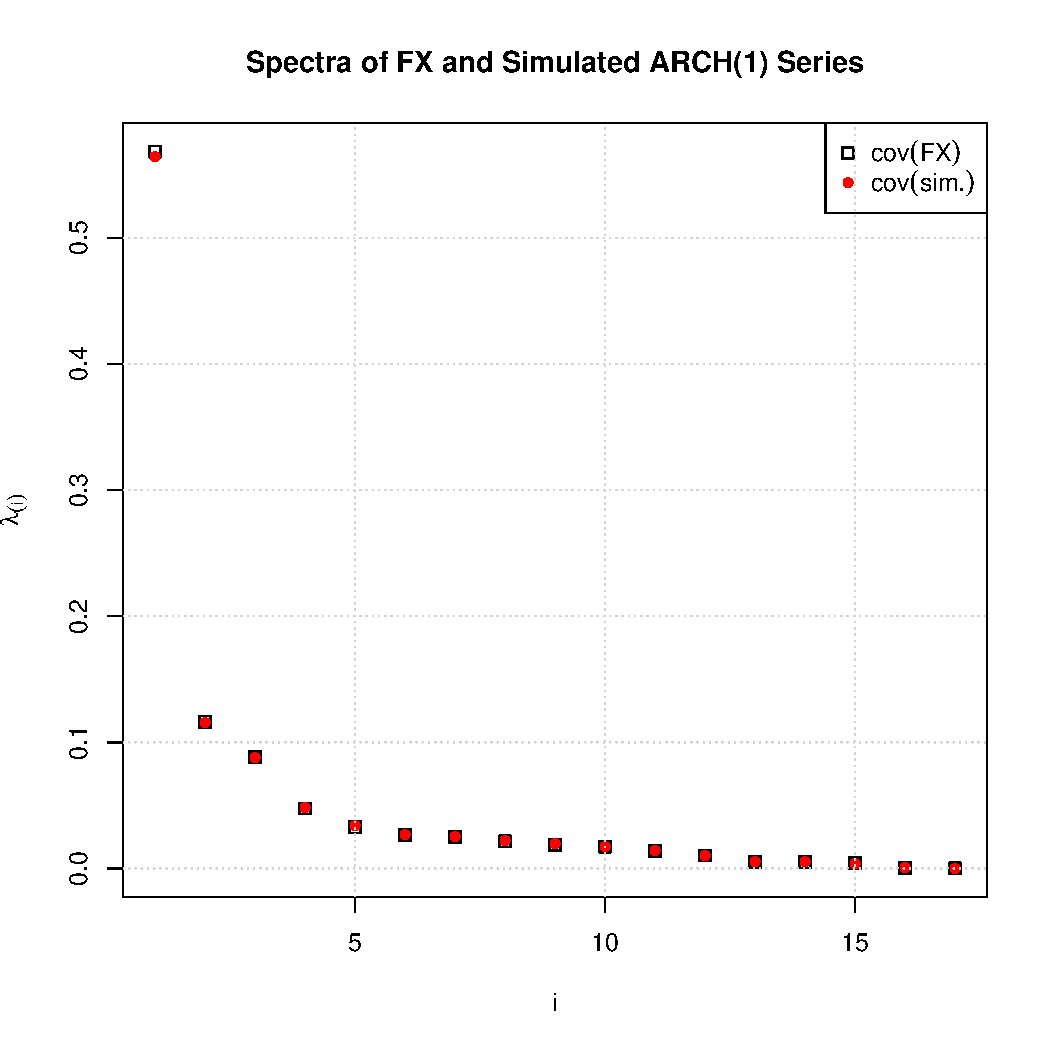
\includegraphics[scale=0.35]{FX_ARCH_eigenvalues.pdf}
    \caption{\tiny Eigenvalues of real FX series and simulated ARCH(1) series}
  \end{figure}
\end{frame}

\begin{frame}
  \begin{figure}[htb!]
    \centering
    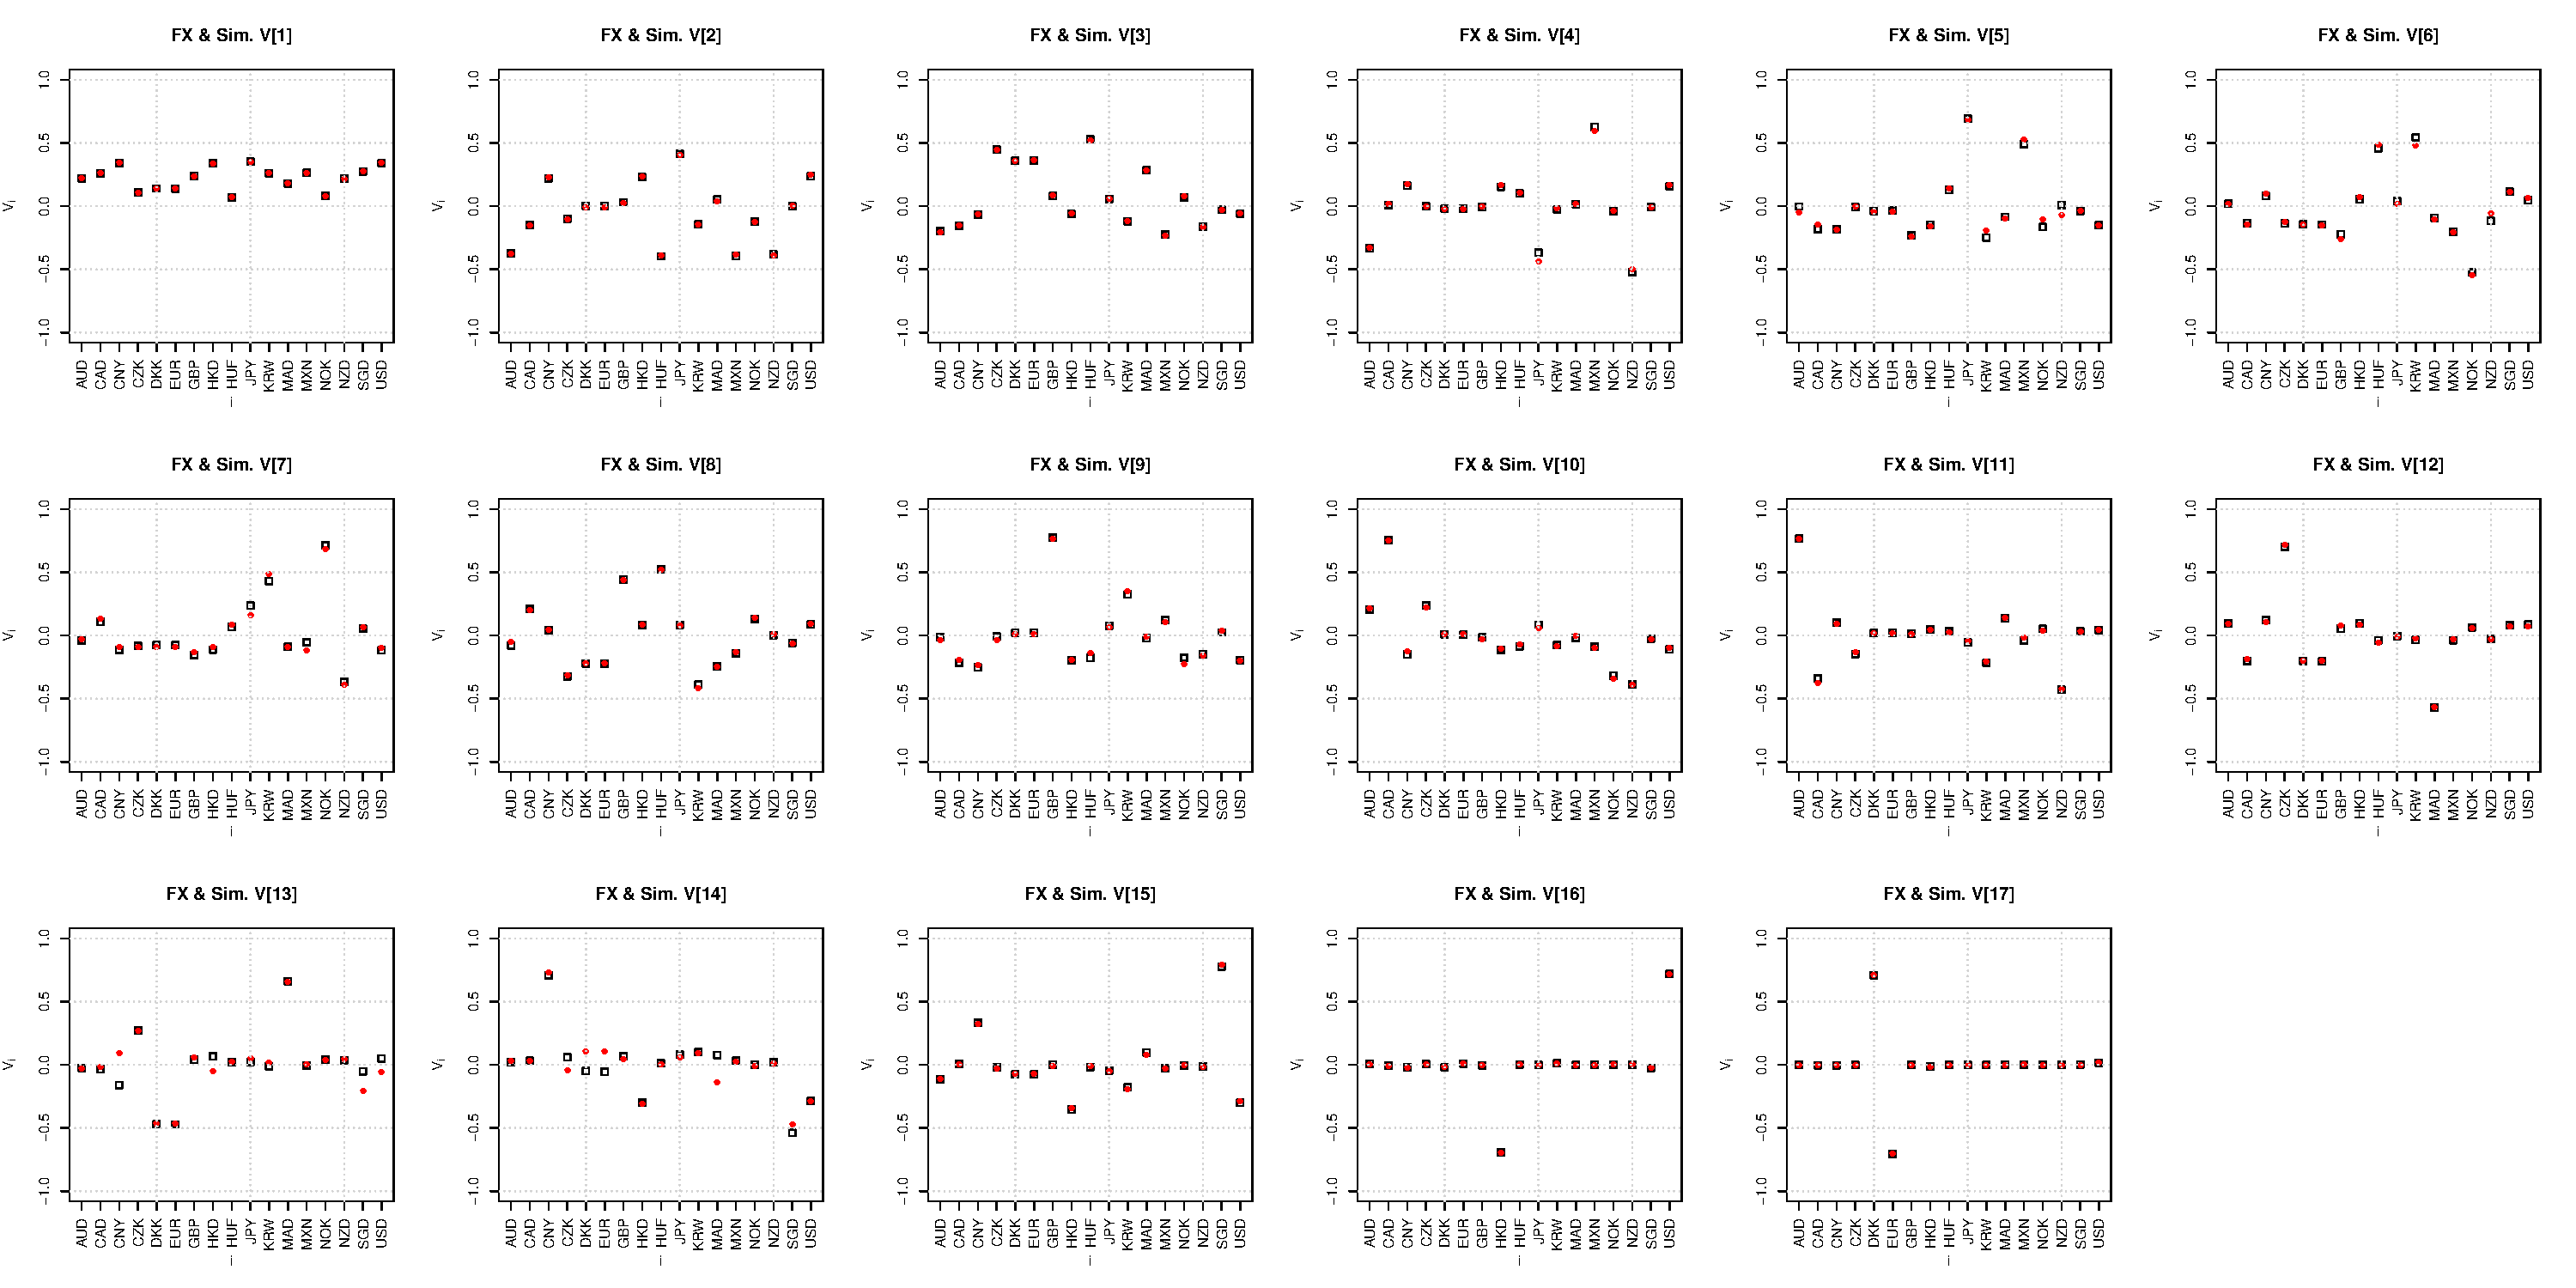
\includegraphics[scale=0.2]{FX_ARCH_eigenvectors.pdf}
    \caption{\tiny Eigenvectors of real FX series and simulated ARCH(1) series}
  \end{figure}
\end{frame}

\begin{frame}
  \frametitle{General IGARCH(1)}
  For general IGARCH(1) models, $\kappa_{i,j}$ as the solution to
  \begin{equation*}
    \E \left[
      (
      \alpha_i Z_1^2 + 1 - \alpha_i
      )^\xi
      (
      \alpha_j Z_2^2 + 1 - \alpha_j
      )^\xi\right] = 1
  \end{equation*}
  can be solved numerically.
  % {r}{0.5\textwidth}
  \begin{figure}
    \begin{center}
      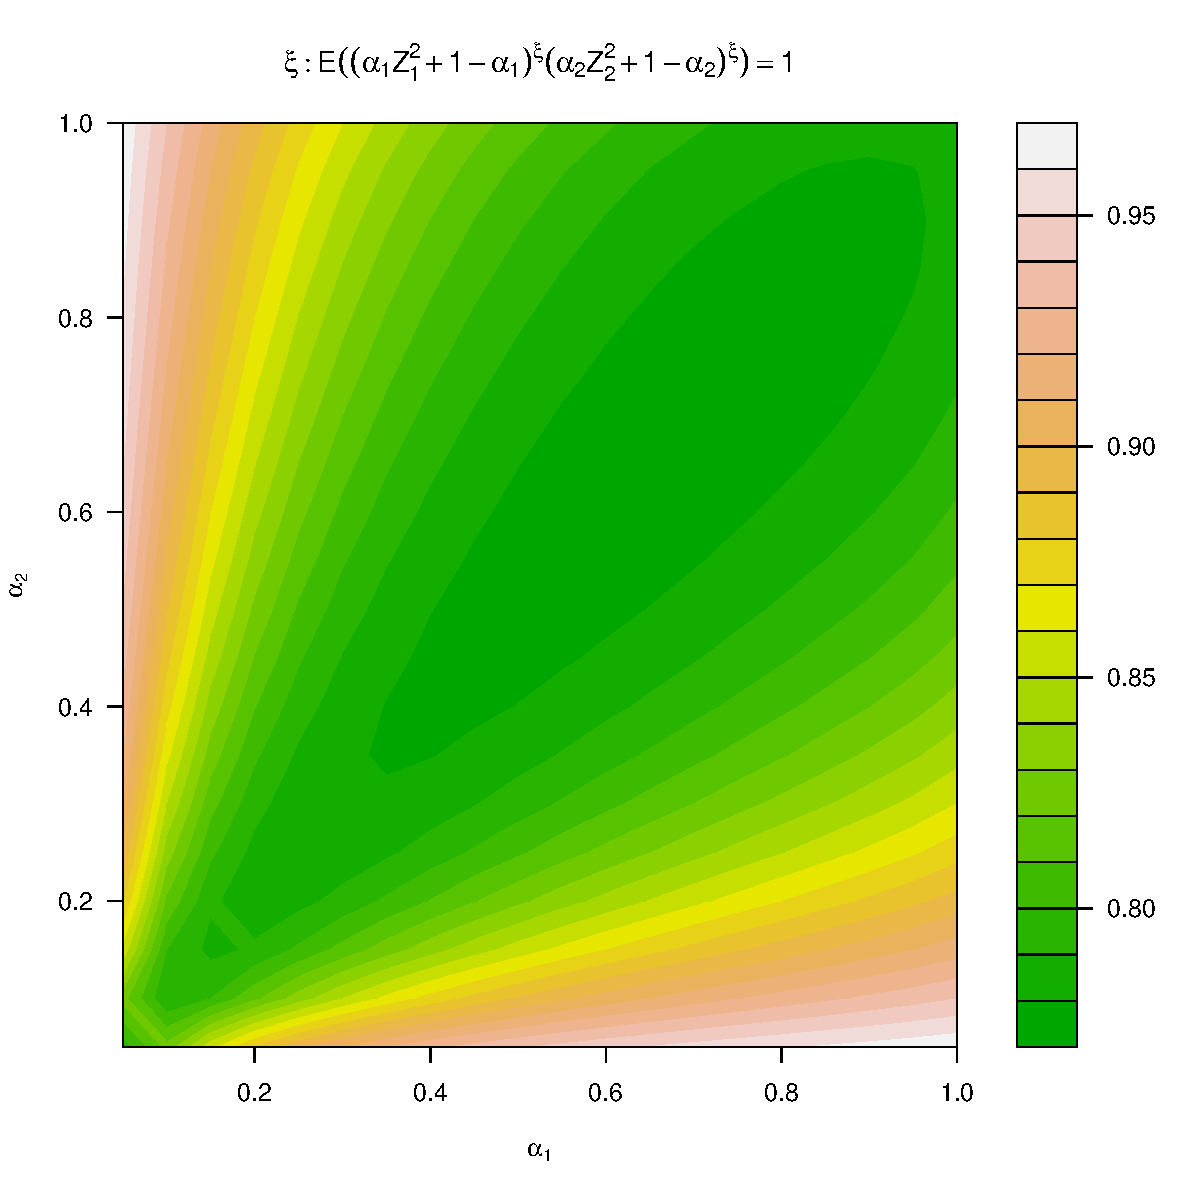
\includegraphics[scale=0.2]{igarch_rho0dot5.pdf}      
    \end{center}
    \label{fig:xi_rho0.5}
    \caption{$\kappa_{i,j}(\alpha_1, \alpha_2)$ for $\text{cov}(Z_1, Z_2) = 1/2$}
  \end{figure}
  $X_{i,t} X_{j,t}$ can have an even heavier tail than does $X_{i,t}^2$ or $X_{j,t}^2$.
\end{frame}

\begin{frame}
  Problems yet to be solved:
  \begin{itemize}
  \item Why the multivariate GARCH/ARCH models give a good fit to the observed eigenvalues \& eigenvectors.
  \item show joint regular variation of
    \[
    \sigma_{1,t}^2, ..., \sigma_{p,t}^2, \{\sigma_{i,t}^2
    \sigma_{j,t}^2\}_{1 \leq i < j \leq p}
    \]
  \end{itemize}
\end{frame}

% \section{GARCH(p,q) Processes}
% \begin{frame}
%   \frametitle{GARCH(p,q) processes}  
%   \begin{eqnarray*}
%     \sigma_{t}^2 &=& \omega + \sum_{i=1}^p \alpha_i X_{t-i}^2 +
%     \sum_{i=1}^q \beta_i \sigma_{t-i}^2 \\
%     X_{i, t} &=& \sigma_{i, t} Z_{i, t} \\
%     Z_{i, t} &\sim& N(0, 1), t(\nu), ...
%   \end{eqnarray*}
%   In this study we assume $Z_{i, t} \sim N(0,1)$.
% \end{frame}

% \begin{frame}
%   \begin{equation*}
%     \begin{tiny}
%       \begin{pmatrix}
%         \sigma_{t}^2 \\
%         \sigma_{t-1}^2 \\
%         \vdots \\
%         \sigma_{t-q+1}^2 \\
%         X_{t-1}^2 \\
%         X_{t-2}^2 \\
%         \vdots \\
%         X_{t-p+1}^2
%       \end{pmatrix} =
%       \begin{pmatrix}
%         \alpha_1 Z_{t-1}^2 + \beta_1 & \beta_2 & \cdots & \beta_q & \alpha_2 & \alpha_3 & \cdots & \alpha_p \\
%         1 & 0 & \cdots & 0 & 0 & 0 & \cdots & 0 \\
%         \vdots & \vdots & \cdots & \vdots & \vdots & \vdots & \cdots & \vdots \\
%         0 & 0 & \cdots & 0 & 0 & 0 & \cdots & 0 \\
%         Z_{t-1}^2 & 0 & \cdots & 0 & 0 & 0 & \cdots & 0 \\
%         0 & 0 & \cdots & 0 & 1 & 0 & \cdots & 0 \\
%         \vdots & \vdots & \cdots & \vdots & \vdots & \vdots & \cdots & \vdots \\
%         0 & 0 & \cdots & 0 & 0 & 0 & \cdots & 0 \\    
%       \end{pmatrix}
%       \begin{pmatrix}
%         \sigma_{t-1}^2 \\
%         \sigma_{t-2}^2 \\
%         \vdots \\
%         \sigma_{t-q}^2 \\
%         X_{t-2}^2 \\
%         X_{t-3}^2 \\
%         \vdots \\
%         X_{t-p}^2
%       \end{pmatrix} +
%       \begin{pmatrix}
%         \omega \\
%         0 \\
%         \vdots \\
%         0 \\
%         0 \\
%         0 \\
%         \vdots \\
%         0 \\
%       \end{pmatrix}
%       \end{tiny}
%     \end{equation*}
%     Compactly
%     \[
%     V_t = A_t V_{t-1} + B
%     \]
%   \end{frame}

%   \begin{frame}
%     \frametitle{Properties of $A_t$}
%     \begin{itemize}
%     \item $\inf_{n \geq 1} {1 \over n}\E \ln \|A_n \cdots A_1\| < 0$
%     \item 
%     \end{itemize}
%   \end{frame}
%   \begin{frame}
%     \frametitle{GARCH(p,q) processes}
%     By Kesten's  theorem, this matrix recurrence equation has a
%     stationary solution and the stationary distribution has regularly
%     varying tail:
%     \[
%     \lim_{u \to \infty} u^{-\kappa} P(\inn{x, V_t} > u) = C,\; x \in \mathbb S^{d-1}
%     \]
%     where $d = p + q -1$
%   \end{frame}

%   \begin{frame}
%     \frametitle{The tail index $\kappa$}
%     \begin{itemize}
%     \item Needed for risk management
%     \item Needed for Importance sampling of the small probability $P(\inn{x, V_t}
%       > u)$ for large $u$. $\kappa$ is the optimal parameter in
%       changing the measure of $A_t$.
%     \item Difficult to estimate. Defined by
%       \begin{equation*}
%         \lim_{n \to \infty} {1 \over n} \ln \E \|A_n \cdots A_1\|^\kappa
%         = 0
%       \end{equation*}
%       \begin{equation*}
%         \lim_{n \to \infty} \|A_n \cdots A_1 \| = 0
%       \end{equation*}
%     \end{itemize}
%   \end{frame}

%  \begin{frame}
%    \frametitle{How to estimate $\kappa$ -- Resampling}
%     By Kesten(1973),
%     \[
%     \lim_{n \to \infty} {
%       |A_n \cdots A_1 \vec{x}|
%       \over
%       \|A_n \cdots A_1\|
%     } = 1
%     \]
%     for an arbitrary $\vec x \in S^{d-1}$. Introduce
%     \begin{eqnarray*}
%       E_n &=& {
%         A_n \cdots A_1 \vec{x}
%         \over
%         |A_n \cdots A_1 \vec{x}|
%       }
%     \end{eqnarray*}
%     Re-write
%     \begin{eqnarray*}
%       && |A_n \cdots A_1 \vec{x}|^\kappa      \\
%       &=& |A_n E_{n-1}|^\kappa |A_{n-1} \cdots A_1 \vec{x}|^\kappa \\
%       &=& \prod_{i=1}^n |A_i E_{i-1}|^\kappa \\
%     \end{eqnarray*}
%     Apply re-sampling that favors $E_{i-1}$ that is associated with
%     large $| A_{i-1} \cdots A_1 E_0 |^\kappa$.
%  \end{frame}

%  \begin{frame}
%    \frametitle{Algorithm for estimating $\kappa$}
%    First estimate
%    \[
%    \Lambda(\theta) = 
%    \lim_{n \to \infty} {1 \over n}\ln
%    \E \|A_n \cdots A_1\|^\theta
%    \]
%    for any given $\theta > 0$. Then find $\kappa$ by solving
%    $\Lambda(\kappa) = 0$.
%  \end{frame}

%  \begin{frame}
%    \frametitle{Algorithm for estimating $\kappa$}
%    \begin{figure}[htb!]
%      \centering
%      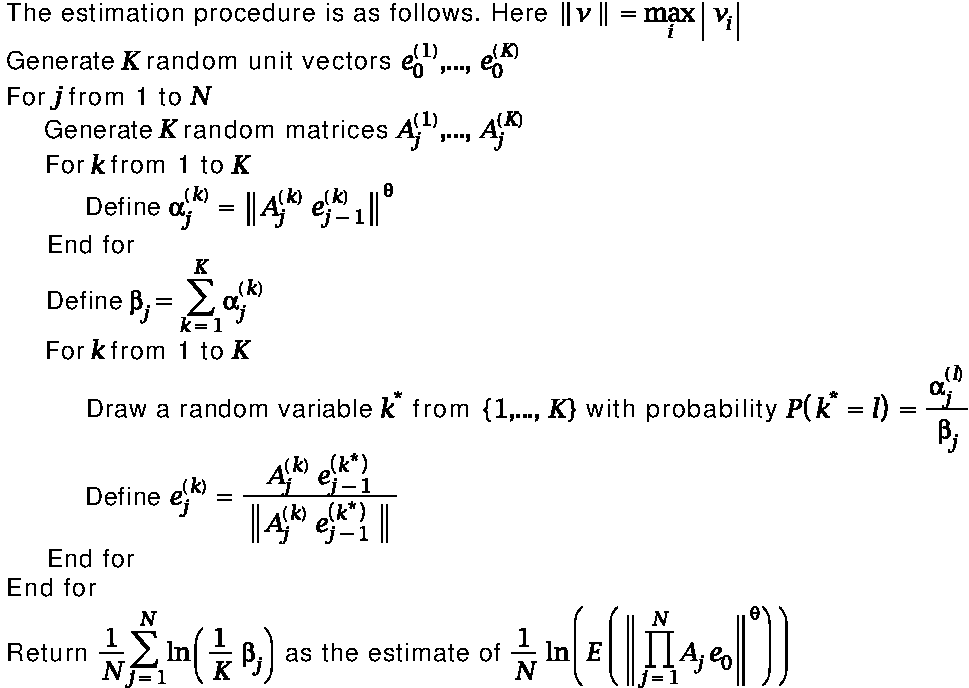
\includegraphics[scale=0.5]{PseudoCode.pdf}
%      % \caption{Pseudo Code for $\kappa$ estimation}
%      \label{fig:PseudoCode}
%    \end{figure}
%  \end{frame}

%  \begin{frame}
%    \frametitle{Algorithm for estimating $\kappa$}
%    \begin{figure}[htb!]
%      \centering
%      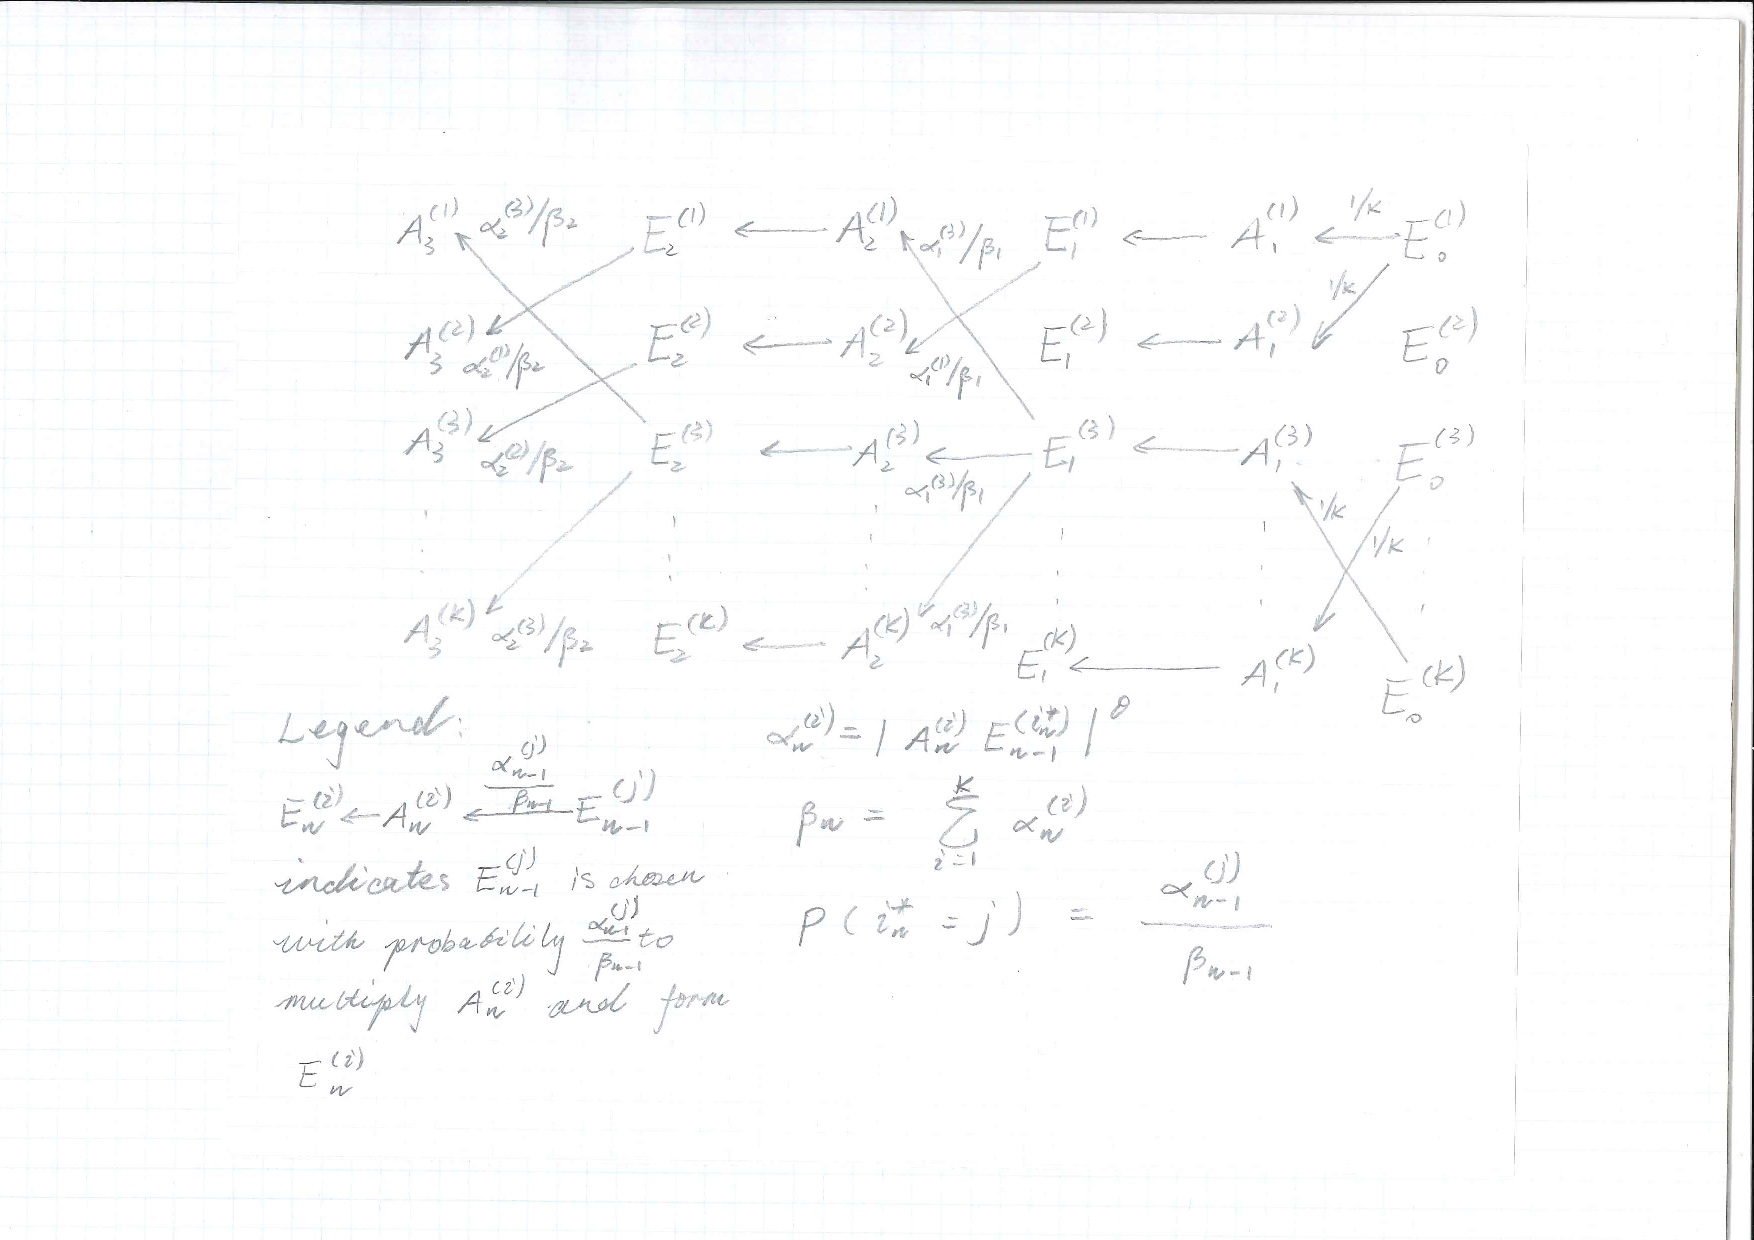
\includegraphics[scale=0.5, trim={4.5cm 0cm 4.5cm 3cm}, clip]{AnandsEstimator.pdf}
%      % \caption{Pseudo Code for $\kappa$ estimation}
%      \label{fig:PseudoCode}
%    \end{figure}
%  \end{frame}

%  \begin{frame}
%    \frametitle{Estimation Results}
%    \begin{minipage}{0.5\linewidth}
%    \begin{figure}[htb!]
%      \centering
%      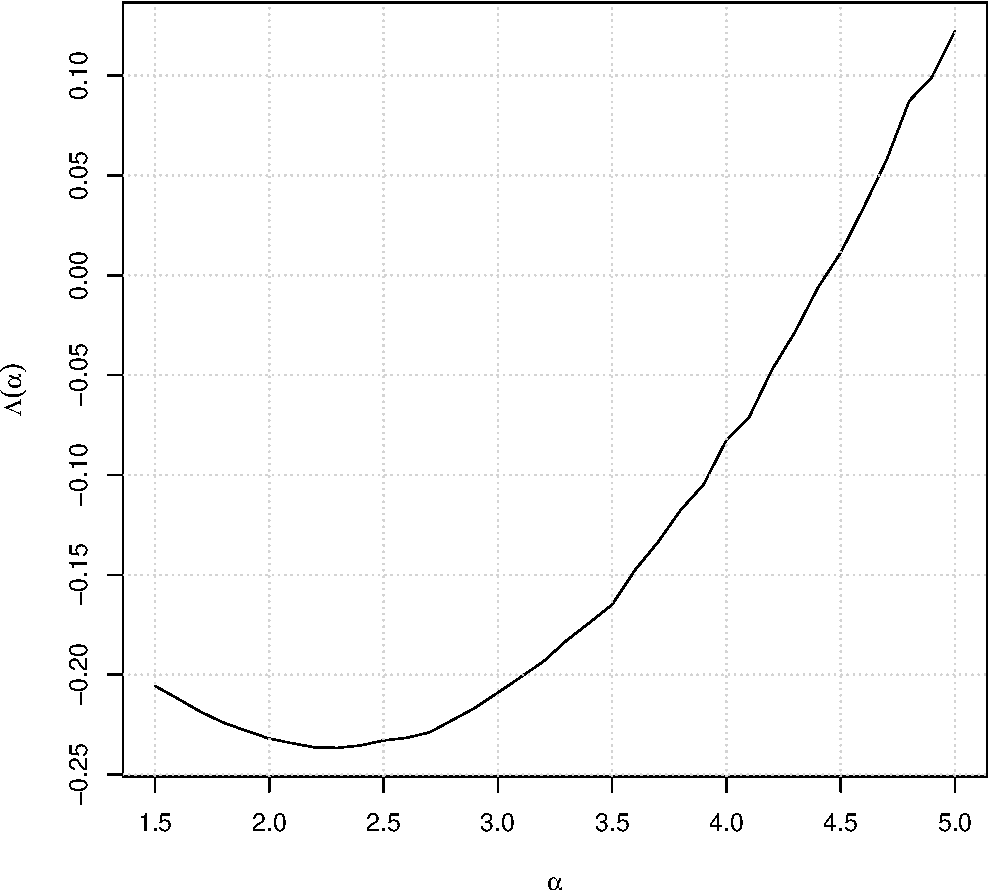
\includegraphics[width=\linewidth]{Lambda.pdf}     
%      \caption{\tiny $\Lambda(\alpha)$ of S\&P 500 modeled as GARCH(2,1)}
%      \label{fig:SP500_Lambda}
%    \end{figure}
%    \end{minipage}\hfill
%    \begin{minipage}{0.5\linewidth}
%      \begin{figure}[htb!]
%        \centering
%        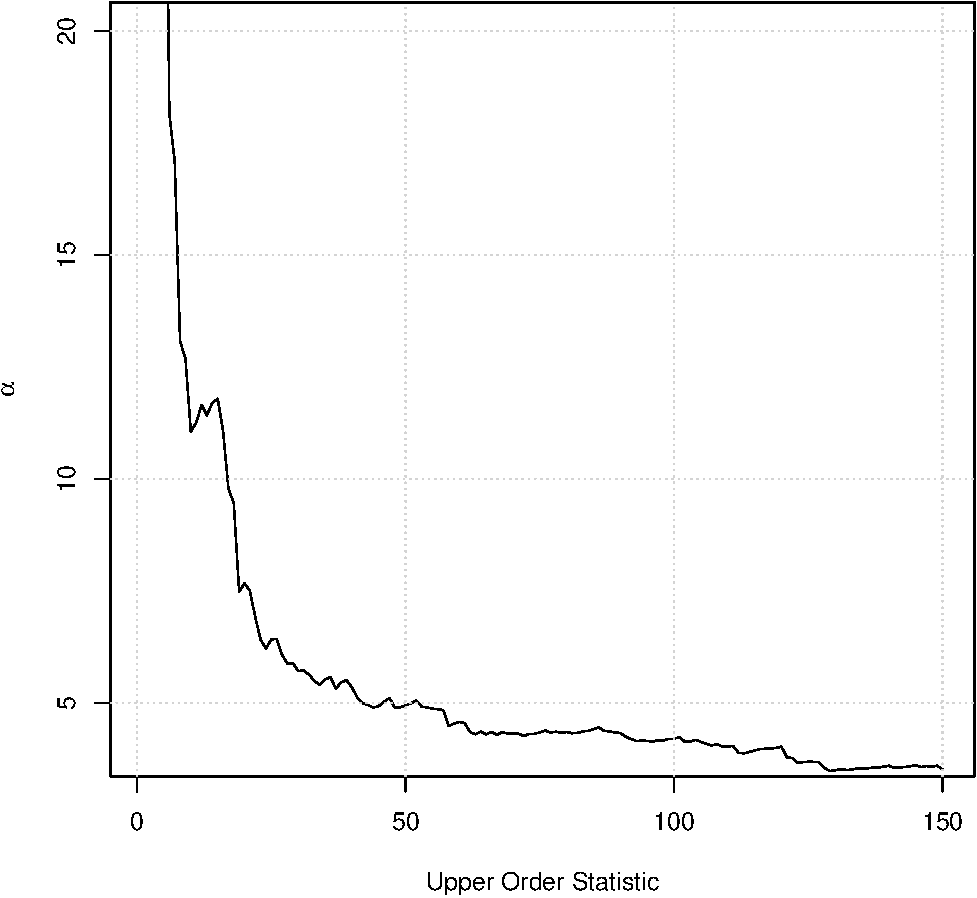
\includegraphics[width=\linewidth]{SP500_var_HillPlot.pdf}
%        \caption{S\&P 500 $\sigma_t^2$ Hill Plot}
%        \label{fig:SP500_var_HillPlot}
%      \end{figure}
%    \end{minipage}

%    \begin{itemize}
%    \item $\kappa$ = 4.4397
%    \item Hill estimator: 4.3372.
%    \item GARCH(1,1): 4.4465.
%    \end{itemize}
%  \end{frame}
\section{Monte Carlo Estimation of prob. of Large Exceedances}
% \begin{frame}
%   \frametitle{Examples}
%     GARCH(1,1) a typical example of a forward sequence.
%     \begin{eqnarray*}
%       X_n &=& \sigma_n Z_n\\
%       \sigma_n^2 &=& \omega + \alpha_1 X_{n-1}^2 + \beta_1 \sigma_{n-1}^2
%     \end{eqnarray*}
%     In this case
%     \[
%     \sigma_n^2 = f_{Y_n} (\sigma_{n-1}^2) =
%     (\beta_1 + \alpha_1 z_{n-1}^2) \sigma_{n-1}^2
%     + \omega
%     \]
%     Let $V = \lim_{n \to \infty} \sigma_n^2$, then
%     \begin{eqnarray*}
%       V &\overset{d}{=}& (\beta_1 + \alpha_1 z^2) V + \omega
%     \end{eqnarray*}
%     By Kesten-Goldie theorem
%     \[
%     \lim_{u \to \infty} u^{\kappa} \P(V > u) = C
%     \]
% \end{frame}

\begin{frame}
  \frametitle{Agenda}
  \begin{itemize}
    \item \textcolor[HTML]{AAAAAA}{A Multivariate GARCH Model with Correlated Innovations}
      \begin{enumerate}
      \item \textcolor[HTML]{AAAAAA}{Empirical eigen structure fitted to financial data}
      \item \textcolor[HTML]{AAAAAA}{Theory of the eigen structure.}
      \end{enumerate}
  \item Stochastic Recurrence Equations, e.g. GARCH(p,q): Monte Carlo
    estimation of probabilities of large exceedances.
    \begin{enumerate}
    \item Importance sampling estimator in 1D
    \item Extension to multi-dimensions
    \end{enumerate}
  \end{itemize}
\end{frame}

\begin{frame}
  \frametitle{Importance Sampling Estimator}
  \underline{\scriptsize{Assume $X$ has prob. density function $f$. Want to estimate $\P(X
  > u) = \E \1{X > u}$:}}

  \begin{minipage}[t]{0.45\linewidth}
    \textcolor[HTML]{990033}{Naive Monte Carlo}
    \begin{scriptsize}
      \begin{eqnarray*}
        \E \1{X > u} &=& \int \1{X > u} f(x) dx
      \end{eqnarray*}
      Draw $n$ iid samples of $X$ from $f(x)$, say $x_1, ..., x_n$,
      then estimate $\P(X > u)$ as
      \[
      {1 \over n} \sum_{i=1}^n \1{x_i > u}
      \]
    \end{scriptsize}
  \end{minipage}\hfill
  \begin{minipage}[t]{0.5\linewidth}
    \textcolor[HTML]{990033}{Importance Sampling}
    \begin{scriptsize}
      \begin{eqnarray*}
        \E \1{X > u} &=& \int \lambda(\kappa)\1{X > u} e^{-\kappa x}
                         {e^{\kappa x} f(x) \over \lambda(\kappa)} dx
      \end{eqnarray*}
      where
      \[
      \lambda(\kappa) = \int e^{\kappa x} f(x) dx < \infty
      \]
      So
      \[
      f_\kappa(x) = \frac{e^{\kappa x} f(x)}{\lambda(\kappa)}
      \]
      is a density function. Draw $x_1, ..., x_n$ from
      $f_\kappa(x)$ and estimate $\P(X > u)$ as
      \[
      {1\over n}\sum_{i=1}^n \lambda(\kappa) \1{x_i > u} e^{-\kappa x_i}
      \]
      \bf{One can show $\kappa$ for which
        $\lambda(\kappa) = 1$ minimises the relative error of the
        estmator.}
    \end{scriptsize}
  \end{minipage}
\end{frame}

\begin{frame}
  \frametitle{GARCH(1,1) prob. of Large Exceedance}
  Want to estimate $\P(\sigma_t^2 > u)$ for large $u$. $\sigma_t^2
  \sim \pi$, the stationary distribution of $\sigma_t^2$.
  \begin{eqnarray*}
    \sigma_t^2 &=& \alpha X_{t-1}^2 + \beta \sigma_{t-1}^2 + \omega \\
               &=& (\alpha Z_{t-1}^2 + \beta) \sigma_{t-1}^2 + \omega
    \\
               &=& A_t \sigma_{t-1}^2 + \omega
  \end{eqnarray*}
   Intuitively
   \[
   \P(\sigma^2_t > u) = {
     \E_\gamma N_u
     \over
     \E_\gamma K
   }
   \]
   where
   \begin{footnotesize}
     \begin{itemize}
     \item $K$ is the typical length of a cycle: Suppose $\sigma_0^2 \in
       (0, M]$, $K > 0$ is the first time when $\sigma_K^2 \in
       (0, M]$. $K$ is random.
     \item $\sigma_0^2 \in (0, M]$ and $\sigma_0^2 \sim \gamma$,
       $\gamma(E) = \pi(E) / \pi((0, M])$, for all $E \subseteq (0,
       M]$.
     \item
       \[
       N_u = \sum_{i=0}^{K - 1} \1{\sigma^2_i > u}
       \]
     \item $\E_\gamma$: Start the process with $\sigma_0^2 \sim
       \gamma$. Take the expectation w.r.t. $\pi$.
     \end{itemize}
   \end{footnotesize}
   % where  and
   % It is straight forward to show $\E K = 1/\pi(\mathcal C)$. We need to
   % have an efficient estimator for $\E N_u$.
 \end{frame}

 \begin{frame}
   \frametitle{GARCH(1,1) prob. of Large Exceedance}
   Define
   \begin{itemize}
   \item $K_i$: the time when the process visits $(0, M]$ for the
     $i$-th time;
   \item $\mathcal R_n$: Number of visits the process pays to $(0, M]$
     up to time $n$.
   \end{itemize}
   By law of large numbers for Markov chains (LLN):
   \begin{eqnarray*}
     \E_\gamma N_u &=& \lim_{m \to \infty} {1 \over m} \sum_{i=1}^m
                       \sum_{t=K_{i-1}}^{K_i - 1} \1{V_t > u} \\
                   &=& \lim_{m \to \infty} {1 \over m} \sum_{t=0}^{K_m
                       - 1} \1{V_t > 0}
   \end{eqnarray*}
   Also by LLN,
   \begin{eqnarray*}
     \P(\sigma_t^2 > u) &=& \lim_{n \to \infty} {1 \over n} \sum_{t=0}^n \1{\sigma_t^2 > u} \\
     &=& \lim_{n \to \infty}{1 \over n} \left[
         \sum_{t=0}^{K_{\mathcal R_n} - 1} \1{\sigma_t^2 > u}
         +
         \sum_{t=K_{\mathcal R_n}}^{n} \1{\sigma_t^2 > u}
         \right]
   \end{eqnarray*}
 \end{frame}

\begin{frame}
  \frametitle{GARCH(1,1) prob. of Large Exceedance}
  \[
  \P(\sigma_t^2 > u) =
  \lim_{n \to \infty} {1 \over n} \sum_{t=0}^{K_{\mathcal R_n} - 1} \1{\sigma_t^2 > u}
  +
  \lim_{n \to \infty} {1 \over n}\sum_{t=K_{\mathcal R_n}}^{n} \1{\sigma_t^2 > u}
  \]
  By Markov renewal theorem (Iscoe, Ney and Nummelin (1985)) and
  geometric ergodicity of the process, the 2nd sum tends to 0 with
  prob. 1 as $n \to \infty$.
  \[
  {1 \over n} \sum_{t=0}^{K_{\mathcal R_n} - 1} \1{\sigma_t^2 > u}
  = {\mathcal R_n \over n} {1 \over \mathcal R_n}
  \sum_{t=0}^{K_{\mathcal R_n} - 1} \1{\sigma_t^2 > u}
  \to \pi((0, M]) \E_\gamma N_u
  \]
  $\{\sigma_t^2 > u\}$ is a rare event, so importance sampling is needed to
  estimate $\E_\gamma N_u$.
  % Let $\mathcal D$ denotes the dual measure:
  % Before the MC exceeds the level $u$, $\log A_{n}$ is sampled from the
  % $\kappa$-shifted distribution $\mu_\kappa$; otherwise it is sampled from
  % $\mu$.
  % \[
  % \mu_\kappa(dx) = e^{x \kappa}\mu(dx)
  % \]
  % For a general change of measure
  % \[
  % \mu_\alpha(dx) = {
  %   e^{\alpha x}\mu(dx)
  %   \over
  %   \lambda(\alpha)
  % }
  % \]
  % where
  % \[
  % \lambda(\alpha) = \int e^{x \alpha} \mu(dx)
  % \]
  % But $\lambda(\kappa) = \E A^\kappa = 1$.
\end{frame}

\begin{frame}
  \frametitle{Importance Sampling for GARCH(1,1)}
  $\sigma_{t}^2$ is a Markov chain. Define
  \begin{itemize}
  \item $\xi_t = \ln A_t$
  \item $S_t = \sum_{i=1}^{t} \xi_i$
  \item $T_u$: first time $\sigma_t^2 > u$
  \end{itemize}
  $(\sigma_t^2, S_t)$ is a Markov Additive process with
  transition kernel $P(x, dy \times d\xi)$. Since $N_u \1{T_u \geq
    K} = 0$
  \begin{footnotesize}
    \begin{eqnarray*}
      \E_\gamma N_u &=& \E_\gamma(N_u\1{T_u < K}) \\
      &=& \sum_{t=1}^\infty
      \1{K=t}
      \underbrace{
        \int_0^\infty \int_{-\infty}^\infty
        \cdots
        \int_0^\infty \int_{-\infty}^\infty
      }_{t \text{ fold}}
      \underbrace{
        \sum_{i=1}^{t} \1{x_i > u} \1{T_u < t}
      }_{N_u \1{T_u < t}} \times \\
      &&
      \prod_{i=1}^{t} P(x_{i-1}, d x_{i} \times d\xi_{i})\\
      &=&
      \sum_{t=1}^\infty
      \1{K=t}
      \int_0^\infty \int_{-\infty}^\infty
      \cdots
      \int_0^\infty \int_{-\infty}^\infty
      \prod_{i=1}^{T_u} \left[
        {e^{\kappa \xi_i} \over \lambda(\kappa)}
        P(x_{i-1}, d x_{i} \times d\xi_{i})
        \right] \times \\
      &&
      \prod_{i=T_u + 1}^{t} P(x_{i-1}, dx_{i} \times d\xi_i)
      \underbrace{
        e^{-\kappa S_{T_u}} N_u\1{T_u < t} \lambda(\kappa)^{T_u}
      }_{\text{estimator}}
    \end{eqnarray*}
  \end{footnotesize}
\end{frame}

\begin{frame}
  \frametitle{Importance Sampling for GARCH(1,1)}
  Choose $\kappa$ such that $\lambda(\kappa) = 1$.
  \begin{minipage}[t]{0.55\linewidth}
    \begin{figure}
      \centering
      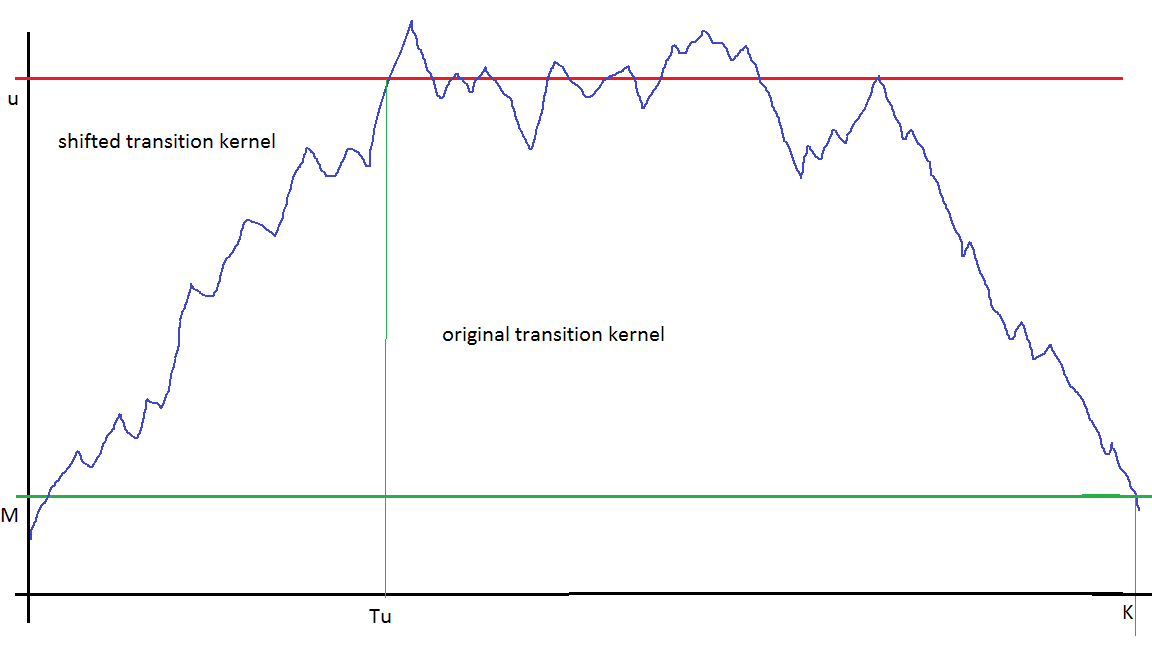
\includegraphics[width=1.0\linewidth]{pic1.png}
      \caption{Dual shift of Transition kernel}
      \label{fig:dual_measure}
    \end{figure}
    \begin{scriptsize}
      Note
      \[
      \int_0^\infty \int_{-\infty}^{\infty}
      e^{\kappa \xi_i}
      P(x_{i-1}, d x_{i} \times d\xi_{i})
      = \E A_i^\kappa = \lambda(\kappa)
      \]
      So
      \[
      {e^{\kappa \xi_i} \over \lambda(\kappa)}
      P(x_{i-1}, d x_{i} \times d\xi_{i})
      \]
      is a transition kernel.
    \end{scriptsize}
  \end{minipage}\hfill
  \begin{minipage}[t]{0.4\linewidth}
    \begin{scriptsize}
      Algorithm:
      \begin{enumerate}
      \item draw $\sigma_0^2$ according to $\gamma$
      \item Simulate the Markov chain according to the shifted transition
        kernel
        \[
        {e^{\kappa \xi_i} \over \lambda(\kappa)}
        P(x_{i-1}, d x_{i} \times d\xi_{i})
        \]
        until $\sigma_t^2 > u$. Then set $N_u = 1$.
      \item Continue to simulate the chain according to $P(x_{i-1}, d
        x_{i} \times d\xi_{i})$ until $\sigma_t^2 \in (0, M]$. Increase $N_u$
        each time $\sigma_t^2 > u$.
      \end{enumerate}
    \end{scriptsize}
  \end{minipage}
\end{frame}

\begin{frame}
  \frametitle{GARCH(p,q) processes}
  \begin{tiny}
    \begin{equation*}
      \begin{pmatrix}
        \sigma_{t}^2 \\
        \sigma_{t-1}^2 \\
        \vdots \\
        \sigma_{t-q+2}^2 \\
        \sigma_{t-q+1}^2 \\
        X_{t-1}^2 \\
        X_{t-2}^2 \\
        \vdots \\
        X_{t-p+2}^2 \\
        X_{t-p+1}^2
      \end{pmatrix} =
      \begin{pmatrix}
        \alpha_1 Z_{t-1}^2 + \beta_1 & \beta_2 & \cdots &
        \beta_{q-1} & \beta_q & \alpha_2 & \alpha_3 & \cdots & \alpha_p & 0 \\
        1 & 0 & \cdots & 
        0 & 0 & 0 & 0 & \cdots & 0 & 0 \\
        \vdots & \vdots & \ddots & 
        \vdots & \vdots & \vdots & \vdots & \ddots & \vdots & \vdots \\
        0 & 0 & \cdots &
        0 & 0 & 0 & 0 & \cdots & 0 & 0 \\
        0 & 0 & \cdots &
        1 & 0 & 0 & 0 & \cdots & 0 & 0 \\
        Z_{t-1}^2 & 0 & \cdots &
        0 & 0 & 0 & 0 & \cdots & 0 & 0 \\
        0 & 0 & \cdots &
        0 & 0 & 1 & 0 & \cdots & 0 & 0 \\
        \vdots & \vdots & \ddots &
        \vdots & \vdots & \vdots & \vdots & \ddots & \vdots & \vdots \\
        0 & 0 & \cdots &
        0 & 0 & 0 & 0 & \cdots & 0 & 0 \\    
        0 & 0 & \cdots &
        0 & 0 & 0 & 0 & \cdots & 1 & 0 \\    
      \end{pmatrix}
      \begin{pmatrix}
        \sigma_{t-1}^2 \\
        \sigma_{t-2}^2 \\
        \vdots \\
        \sigma_{t-q+1}^2 \\
        \sigma_{t-q}^2 \\
        X_{t-2}^2 \\
        X_{t-3}^2 \\
        \vdots \\
        X_{t-p+1}^2 \\
        X_{t-p}^2
      \end{pmatrix} +
      \begin{pmatrix}
        \omega \\
        0 \\
        \vdots \\
        0 \\
        0 \\
        0 \\
        0 \\
        \vdots \\
        0 \\
        0 \\
      \end{pmatrix}
    \end{equation*}
  \end{tiny}
    Compactly
    \[
    V_t = A_t V_{t-1} + B
    \]
    By Kesten-Goldie theorem:
    \[
    \lim_{u \to \infty} u^{\kappa} P(\inn{x, V_t} > u) = C \quad x \in \mathbb S^{d-1}
    \]
    where $d = p + q -1$
\end{frame}

\begin{frame}
  \frametitle{GARCH(p,q) processes}
  \begin{scriptsize}
    Want to simulate the rare event prob. by importance sampling
    \[
    \P(|V_t| > u) \quad u \to \infty  
    \]
    Differences from GARCH(1,1):
    \begin{itemize}
    \item Instead of $(0, M]$, define
      \[
      \mathcal C = \{\vec v \in \mathbb R_+^{p+q-1}, |\vec v| \leq M\}
      \]
    \item Define
      \begin{eqnarray*}
        \vec M_t &=& A_{t} \cdots A_1 \vec V_0 \over |A_{t} \cdots A_1 \vec V_0| \\
        S_t &=& \ln |A_t \cdots A_1 \vec V_0| \\
        \xi_t &=& S_t - S_{t-1} =
                  \ln \left|A_t
                  \underbrace{
                  {A_{t-1} \cdots A_1 \vec V_0 \over |A_{t-1} \cdots A_1 \vec V_0|}
                  }_{M_{t-1}}
                  \right|
      \end{eqnarray*}
      $(\vec M_t, S_t)$ is a Markov Additive process.
    \end{itemize}
  \end{scriptsize}
\end{frame}

\begin{frame}
  \frametitle{GARCH(p,q) processes}
  As in the GARCH(1,1) case,
  \begin{eqnarray*}
    \P(|V_t| > u) &=& \pi(\mathcal C) \E_\gamma(N_u) \\
    N_u &=& \sum_{i=1}^{K-1} \1{|\vec V_t| > u}
  \end{eqnarray*}
  \begin{itemize}
  \item Knowing $\vec V_{t-1}$, $\vec V_t$ is a function of $A_t$
  \item $A_t$ is determined by $\vec M_t$, $\xi_t$ and $\vec M_{t-1}$ via
    \begin{eqnarray*}
      e^{\xi_t} \vec M_t &=& A_t \vec M_{t-1}
    \end{eqnarray*}
    Observe $A_t$ is determined by $Z_{t-1}^2$, which is given by
    \[
    Z_{t-1}^2 = {
      \inn{\vec e_{q+1}, e^{\xi_t} \vec M_{t}}
      \over
      \inn{\vec e_{1}, \vec M_{t-1}}
    }
    \]
  \end{itemize}
  \underline{$\vec V_t$ is a function of $\vec M_t$, $\xi_t$ and $\vec M_{t-1}$}
\end{frame}

\begin{frame}
  \frametitle{Importance Sampling for GARCH(p,q)}
  \begin{itemize}
  \item Define operator $T$ on a function $f \in \mathscr C_b(\mathbb
    S^{d-1}_+)$, i.e. continuous and bounded functions defined on the
    positive unit sphere.
    \[
    T_\kappa f(\vec x) = \int |A \vec x|^\kappa
    f\left({A \vec x \over |A \vec x|}\right) \mu(dA)
    \]
  \item Define right eigen function $r_\kappa \in \mathscr C_b(\mathbb
    S^{d-1}_+)$, and eigenvalue $\lambda(\kappa)$ by
    \[
    (T_\kappa r_\kappa)(\vec x) = \lambda(\kappa) r(\vec x)
    \]
  \item $Q(\vec x_{i-1}, d\vec x_{i} \times d\xi_{i})$: transition kernel of
    $(\vec M_t, S_t)$. Since $\vec x_i$ and $\xi_i$ denpend only on
    $A_i$
    \begin{scriptsize}
      \begin{eqnarray*}
        && \int_{\mathbb S_+^{d-1}} \int_{-\infty}^\infty
        {e^{\kappa \xi_i} \over \lambda(\kappa)}
        {r_\kappa(\vec x_i) \over r_\kappa(\vec x_{i-1})}
        Q(x_{i-1}, d\vec x_{i} \times d\xi_{i}) \\
        &=&
        {1 \over \lambda(\kappa) r_\kappa(\vec x_{i-1})}
        \int |A_i \vec M_{i-1}|^\kappa
        r_\kappa\left(
          { A_i \vec x_{i-1}
            \over
            |A_i \vec x_{i-1}|
          }
        \right) \mu(dA) \\
        &=& 
        {1 \over \lambda(\kappa) r_\kappa(\vec x_{i-1})}
        (T_\kappa r_\kappa)(\vec x_{i-1}) \\
        &=& 1
      \end{eqnarray*}
    \end{scriptsize}
  \end{itemize}
  % \frametitle{An Efficient Estimator}
  %   \[
  %   \mathcal E_u = \pi(\mathcal C) {N_u
  %     \over
  %     (A_{T_u} \cdots A_1)^\kappa
  %   }\1{T_u < K}
  %   \]
  %   is an efficient estimator of $\P(V > u)$, meaning 
  % \begin{eqnarray*}
  %   \E_{\mathcal D}(\mathcal E_u) &=& \P(V > u) \\
  %   \sup_{u > 0} {
  %     \var_{\mathcal D}(\mathcal E_u)
  %     \over
  %     (\E_{\mathcal D} \mathcal E_u)^2
  %   } &\leq& C
  % \end{eqnarray*}
  % for some constant C.
\end{frame}

\begin{frame}
  \frametitle{Importance Sampling for GARCH(p,q)}
  The importance sampling estimator can now be found:
  \begin{scriptsize}
    \begin{eqnarray*}
      && \E_\gamma (N_u \1{T_u < K}) \\
      &=&
      \sum_{t=1}^\infty \1{K=t}
      \left[
        \underbrace{
          \int_{\mathbb S_+^{d-1}} \int_{-\infty}^\infty
          \cdots
          \int_{\mathbb S_+^{d-1}} \int_{-\infty}^\infty
        }_{t\ \text{fold}}
        \underbrace{
          N_u \1{T_u < t} e^{-\kappa S_{T_u}}
          {r_\kappa(\vec x_{0}) \over r_\kappa(\vec x_{T_u})}
          \lambda(\kappa)^{T_u}
        }_{\text{estimator}}
        \times \right.\\ 
        && \left.\prod_{i=1}^{T_u}
               {e^{\kappa \xi_i} \over \lambda(\kappa)}
               {r_\kappa(\vec x_i) \over r_\kappa(\vec x_{i-1})}
               Q(x_{i-1}, d\vec x_{i} \times d\xi_{i})
               \prod_{i=T_u+1}^{t}
               Q(x_{i-1}, d\vec x_{i} \times d\xi_{i})
               \right]
    \end{eqnarray*}
  \end{scriptsize}
  Choose $\kappa$ such that $\lambda(\kappa) = 1$. In multidimensions,
  \[
  \lambda(\kappa) = \lim_{n \to \infty} (\E \|A_n \cdots A_1\|^\kappa)^{1/n}
  \]
\end{frame}

\begin{frame}
  \frametitle{The function $\Lambda(\kappa)$}
  \begin{minipage}{0.5\linewidth}
      \begin{itemize}
      \item 1D:
        \begin{eqnarray*}
          A &=& \alpha Z^2 + \beta \\
          Z &\sim& N(0,1) \\
          \Lambda(\alpha) &=& \ln(\lambda(\kappa)) = \ln \E A^\alpha          
        \end{eqnarray*}
      \item multi-dimension:
        \begin{eqnarray*}
          \Lambda(\alpha) &=& \ln(\lambda(\kappa)) \\
          &=& \lim_{n \to \infty} {1 \over n} \ln \E \|A_n \cdots A_1\|^\alpha
        \end{eqnarray*}
        Estimation of $\kappa$ is trickier than in 1D.
      \end{itemize}
  \end{minipage}\hfill
  \begin{minipage}{0.4\linewidth}
    \begin{figure}
      \centering
      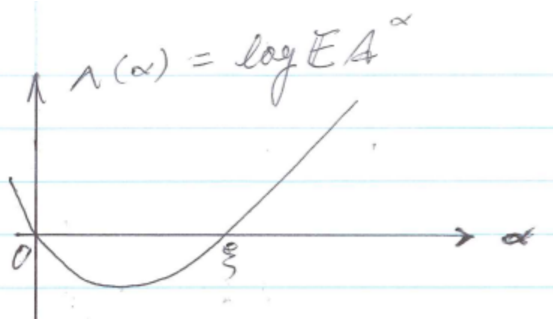
\includegraphics[width=1.0\linewidth]{pic2.pdf}
    \end{figure}
    \begin{scriptsize}
    The function $\Lambda(\alpha)$ is convex, passes through the origin
    and crosses the $\alpha$-axis.
    \end{scriptsize}
  \end{minipage}
\end{frame}


 \begin{frame}
   \frametitle{Estimation Results}
   By an algorithm based on resampling, we have obtained plausible
   estimations. Results on {\bf S\&P 500 index} shown below:
   \begin{minipage}{0.5\linewidth}
   \begin{figure}[htb!]
     \centering
     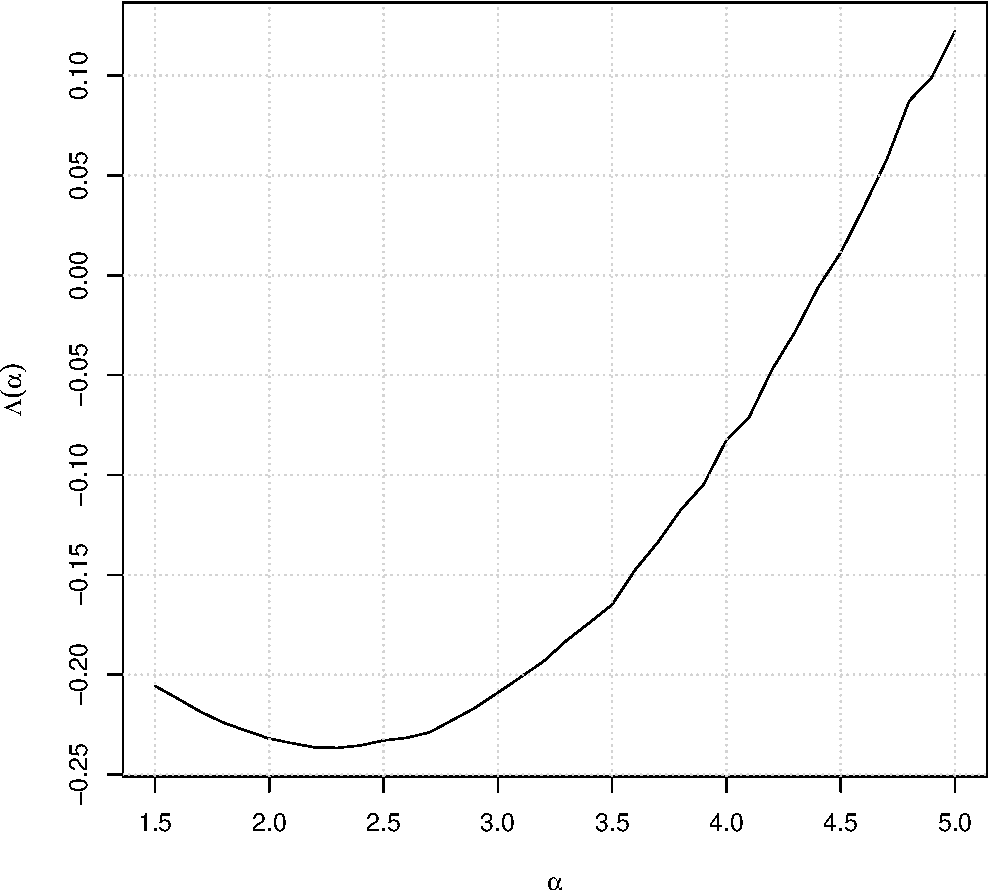
\includegraphics[width=\linewidth]{Lambda.pdf}     
     \caption{\tiny $\Lambda(\alpha)$ of S\&P 500 modeled as GARCH(2,1)}
     \label{fig:SP500_Lambda}
   \end{figure}
   \end{minipage}\hfill
   \begin{minipage}{0.5\linewidth}
     \begin{figure}[htb!]
       \centering
       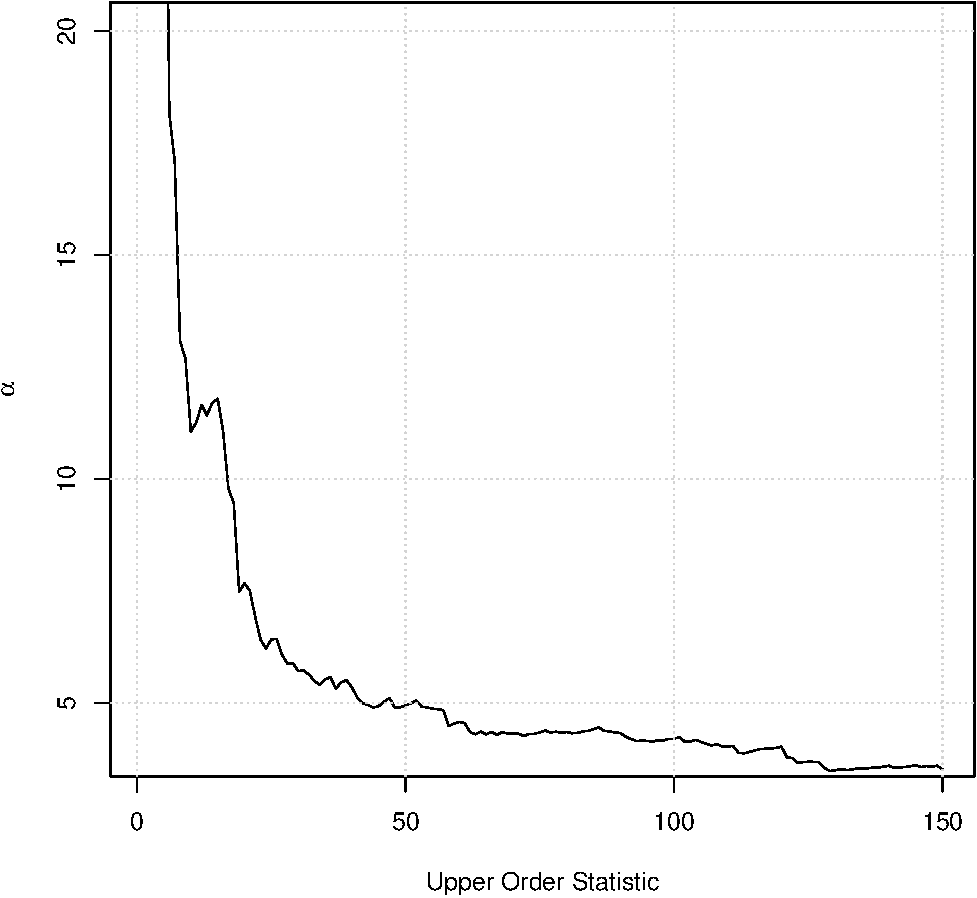
\includegraphics[width=\linewidth]{SP500_var_HillPlot.pdf}
       \caption{S\&P 500 $\sigma_t^2$ Hill Plot}
       \label{fig:SP500_var_HillPlot}
     \end{figure}
   \end{minipage}

   \begin{itemize}
   \item $\kappa$ = 4.4397 when modeled as GARCH(2,1)
   \item $\kappa=4.4465$ when modeled as GARCH(1,1)
   \item Hill estimator: 4.3372.
   \end{itemize}
 \end{frame}

 \begin{frame}
   \frametitle{Thank you!}
   Questions?
 \end{frame}
\bibliographystyle{unsrt}
\bibliography{../../thesis/econophysics}
\end{document} 
